\documentclass[twoside,11pt,a4paper,openany]{book}
\usepackage[amsbb,subscriptcorrection,zswash,mtpcal,mtphrb]{mtpro2}
\usepackage[no-math,cm-default]{fontspec}
\usepackage{xunicode}
\usepackage{xgreek}
\defaultfontfeatures{Mapping=tex-text,Scale=MatchLowercase}
\def\xrwma{black}
\def\xrwmath{black}
\setmainfont[Mapping=tex-text,Numbers=Lining,Scale=1.0]{Minion Pro}
\newfontfamily\mpro{Minion Pro}
\usepackage{amsmath}
\usepackage[left=2.00cm, right=2.00cm, top=3.00cm, bottom=2.00cm]{geometry}
\usepackage{makeidx}
\usepackage{longtable}
\usepackage{etoolbox}
\makeatletter
\newif\ifLT@nocaption
\preto\longtable{\LT@nocaptiontrue}
\appto\endlongtable{%
\ifLT@nocaption
\addtocounter{table}{\m@ne}%
\fi}
\preto\LT@caption{%
\noalign{\global\LT@nocaptionfalse}}
\makeatother
\makeindex
\usepackage{tikz,pgfplots}
\usepackage{tkz-euclide,tkz-fct}
\usepackage{wrapfig}
\usetkzobj{all}
\usepackage{calc}
\usepackage{cleveref}
\usepackage[colorlinks=false, pdfborder={0 0 0}]{hyperref}
\usepackage[framemethod=TikZ]{mdframed}
\newcommand{\ypogrammisi}[1]{\underline{\smash{#1}}}
\usetikzlibrary{backgrounds}
\renewcommand{\thepart}{\arabic{part}}
\definecolor{steelblue}{cmyk}{.7,.278,0,.294}
\definecolor{doc}{cmyk}{1,0.455,0,0.569}
\definecolor{olivedrab}{cmyk}{0.25,0,0.75,0.44}
\usepackage{capt-of}
\usepackage{titletoc}
\usepackage[explicit]{titlesec}
\usepackage{graphicx}
\usepackage{multicol}
\usepackage{multirow}
\usepackage{enumitem}
\usepackage{tabularx}
\usepackage{mathimatika,tkz-tab,gensymb}
\tikzset{>=latex}
\makeatletter
\pretocmd{\@part}{\gdef\parttitle{#1}}{}{}
\pretocmd{\@spart}{\gdef\parttitle{#1}}{}{}
\makeatother
\usepackage[titletoc]{appendix}
\usepackage{fancyhdr}
\pagestyle{fancy}
\fancyheadoffset{0cm}
\renewcommand{\headrulewidth}{\iftopfloat{0pt}{.5pt}}
\renewcommand{\chaptermark}[1]{\markboth{#1}{}}
\renewcommand{\sectionmark}[1]{\markright{\it\thesection\ #1}}
\fancyhf{}
\fancyhead[LE]{\thepage\ $\cdot$\ \scshape\nouppercase{\leftmark}}
\fancyhead[RO]{\nouppercase{\rightmark} $\cdot$\ \thepage}
\fancypagestyle{plain}{%
\fancyhead{} %
\renewcommand{\headrulewidth}{0pt}}

\newcounter{thewrhma}[chapter]
\renewcommand{\thethewrhma}{\thechapter.\arabic{thewrhma}} 
\newcommand{\Thewrhma}[1]{\refstepcounter{thewrhma}{\textbf{\textcolor{\xrwmath}{{\large Θεώρημα\hspace{2mm}\thethewrhma\;}:\;}\hspace{1mm}}} \MakeUppercase{\textbf{#1}}\\}{}

\newcounter{porisma}[chapter]
\renewcommand{\theporisma}{\thechapter.\arabic{porisma}}\newcommand{\Porisma}[1]{\refstepcounter{porisma}\textcolor{black}{\textbf{ΠΟΡΙΣΜΑ\hspace{2mm}\theporisma\hspace{1mm} \MakeUppercase{#1}}}\\}{}

\newcounter{protasi}[chapter]
\renewcommand{\theprotasi}{\thechapter.\arabic{protasi}}\newcommand{\Protasi}[1]{\refstepcounter{protasi}\textcolor{black}{\textbf{ΠΡΟΤΑΣΗ\hspace{2mm}\theprotasi\hspace{1mm} \MakeUppercase{#1}}}\\}{}

\newcounter{methodologia}[chapter]
\renewcommand{\themethodologia}{\thechapter.\arabic{methodologia}}\newcommand{\Methodologia}[1]{\refstepcounter{methodologia}\textcolor{black}{\textbf{MΕΘΟΔΟΣ\hspace{2mm}\themethodologia\hspace{1mm} \MakeUppercase{#1}}}\\}{}

\newcounter{orismos}[chapter]
\renewcommand{\theorismos}{\arabic{orismos}}   
\newcommand{\Orismos}[1]{\refstepcounter{orismos}{\textbf{\textbf{\textcolor{\xrwma}{{\large Ορισμός\hspace{2mm}\thechapter.\theorismos\;}:\;}}}}\hspace{1mm} \MakeUppercase{\textbf{#1}\\}}{}
\usepackage{venndiagram}
%-------- ΣΤΥΛ ΚΕΦΑΛΑΙΟΥ ---------
\newcommand*\chapterlabel{}
\newcommand{\fancychapter}{%
\titleformat{\chapter}
{
\normalfont\Huge}
{\gdef\chapterlabel{\thechapter\ }}{0pt}
{\begin{tikzpicture}[remember picture,overlay]
\node[yshift=-7cm] at (current page.north west)
{\begin{tikzpicture}[remember picture, overlay]
%\node[inner sep=0pt] at ($(current page.north) +			(0cm,-1.38in)$) {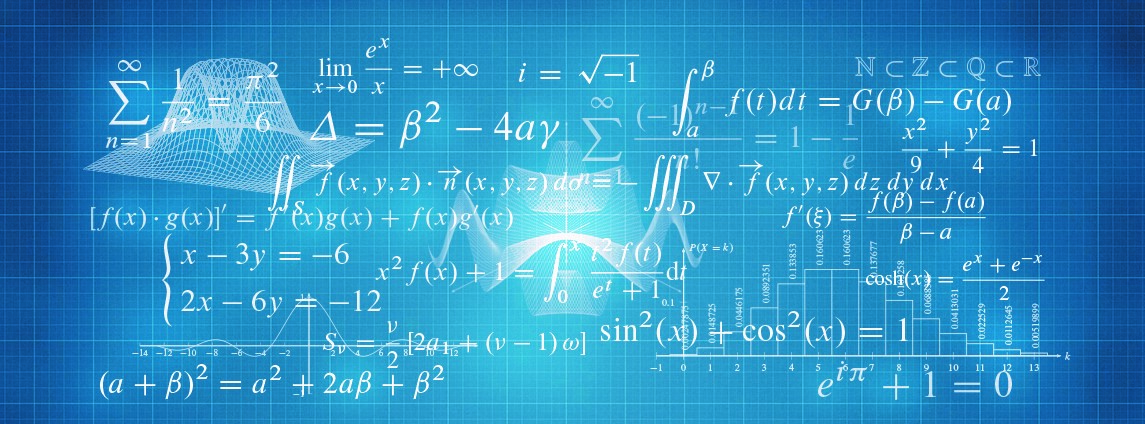
\includegraphics[width=17cm]{Kefalaio}};
\node[anchor=west,xshift=.08\paperwidth,yshift=.1\paperheight,rectangle]
{{\color{white}\fontsize{30}{20}\textbf{\textcolor{black}{\contour{white}{ΚΕΦΑΛΑΙΟ}}}}};
\node[anchor=west,xshift=.07\paperwidth,yshift=.05\paperheight,rectangle] {\fontsize{27}{20} {\color{black}{{\textcolor{black}{\contour{white}{\sc##1}}}}}};
%\fill[fill=black] (12.2,2) rectangle (14.8,4.7);
\node[anchor=west,xshift=.77\paperwidth,yshift=.077\paperheight,rectangle]
{\fontsize{80}{20}\textbf{\textit{\contour{black}{\thechapter}}}};
\end{tikzpicture}
};
\end{tikzpicture}
}
\titlespacing*{\chapter}{0pt}{20pt}{30pt}
}
%------------------------------------------------

\usepackage[outline]{contour}
\newcommand{\regularchapter}{%
\titleformat{\chapter}[display]
{\normalfont\huge\bfseries}{\chaptertitlename\ \thechapter}{20pt}{\Huge##1}
\titlespacing*{\chapter}
{0pt}{-20pt}{40pt}
}

\apptocmd{\mainmatter}{\fancychapter}{}{}
\apptocmd{\backmatter}{\regularchapter}{}{}
\apptocmd{\frontmatter}{\regularchapter}{}{}

\titlespacing*{\section}
{0pt}{30pt}{0pt}
\usepackage{booktabs}
\usepackage{hhline}
\DeclareRobustCommand{\perthousand}{%
\ifmmode
\text{\textperthousand}%
\else
\textperthousand
\fi}

\newcounter{typos}[chapter]
\renewcommand{\thetypos}{T\arabic{typos}}   
\newcommand{\Typos}{\refstepcounter{typos}\textcolor{gray}{\textbf{\thetypos}}}{}


\contentsmargin{0cm}
\titlecontents{part}[-1pc]
{\addvspace{10pt}%
\bf\Large ΜΕΡΟΣ\quad }%
{}
{}
{\;\dotfill\;\normalsize\ Σελίδα}%
%------------------------------------------
\titlecontents{chapter}[0pc]
{\addvspace{30pt}%
\begin{tikzpicture}[remember picture, overlay]%
\draw[fill=black,draw=black] (-.3,.5) rectangle (3.7,1.1); %
\pgftext[left,x=0cm,y=0.75cm]{\color{white}\sc\Large\bfseries Κεφάλαιο\ \thecontentslabel};%
\end{tikzpicture}\large\sc}%
{}
{}
{\hspace*{-2.3em}\hfill\normalsize Σελίδα \thecontentspage}%
\titlecontents{section}[2.4pc]
{\addvspace{1pt}}
{\contentslabel[\thecontentslabel]{2pc}}
{}
{\;\dotfill\;\small \thecontentspage}
[]
\titlecontents*{subsection}[4pc]
{\addvspace{-1pt}\small}
{}
{}
{\ --- \small\thecontentspage}
[ \textbullet\ ][]

\makeatletter
\renewcommand{\tableofcontents}{%
\chapter*{%
\vspace*{-20\p@}%
\begin{tikzpicture}[remember picture, overlay]%
\pgftext[right,x=12cm,y=0.2cm]{\Huge\sc\bfseries \contentsname};%
\draw[fill=black,draw=black] (9.5,-.75) rectangle (12.5,1);%
\clip (9.5,-.75) rectangle (15,1);
\pgftext[right,x=12cm,y=0.2cm]{\color{white}\Huge\bfseries \contentsname};%
\end{tikzpicture}}%
\@starttoc{toc}}
\makeatother
\pgfmathdeclarefunction{gauss}{2}{%
\pgfmathparse{1/(#2*sqrt(2*pi))*exp(-((x-#1)^2)/(2*#2^2))}%
}
\usepackage[contents={},scale=1,opacity=1,color=black,angle=0]{background}

\newcommand\blfootnote[1]{%
\begingroup
\renewcommand\thefootnote{}\footnote{#1}%
\addtocounter{footnote}{-1}%
\endgroup
}
\usepackage{epstopdf}
\epstopdfsetup{update}
\usepackage{textcomp}
\titleformat{\section}
{\normalfont\Large\bf}%
{}{0em}%
{{\color{black}\titlerule[1pt]}\vskip-.2\baselineskip{\parbox[t]{\dimexpr\textwidth-2\fboxsep\relax}{\raggedright\strut\thesection~#1\strut}}}[\vskip 0\baselineskip{\color{black}\titlerule[1pt]}]
\titlespacing*{\section}{0pt}{0pt}{0pt}

\newcommand{\methodologia}{\begin{center}
{\large \textbf{ΜΕΘΟΔΟΛΟΓΙΑ}}\\\vspace{-2mm}
\begin{tikzpicture}
\shade[left color=white, right color=black] (-3cm,0) rectangle (0,.2mm);
\shade[left color=black, right color=white] (0,0) rectangle (3cm,.2mm);   
\end{tikzpicture}
\end{center}}

\newcommand{\orismoi}{\begin{center}
\large \textcolor{\xrwma}{\textbf{ΟΡΙΣΜΟΙ}}\\\vspace{-2mm}
\begin{tikzpicture}
\shade[left color=white, right color=\xrwma] (-3cm,0) rectangle (0,.2mm);
\shade[left color=\xrwma, right color=white] (0,0) rectangle (3cm,.2mm);   
\end{tikzpicture}
\end{center}}
\newcommand{\thewrhmata}{\begin{center}
{\large \textcolor{\xrwmath}{\textbf{ΘΕΩΡΗΜΑΤΑ - ΠΟΡΙΣΜΑΤΑ - ΠΡΟΤΑΣΕΙΣ\\ΚΡΙΤΗΡΙΑ - ΙΔΙΟΤΗΤΕΣ}}}\\\vspace{-2mm}
\begin{tikzpicture}
\shade[left color=white, right color=\xrwmath,] (-5cm,0) rectangle (0,.2mm);
\shade[left color=\xrwmath, right color=white,] (0,0) rectangle (5cm,.2mm);   
\end{tikzpicture}
\end{center}}
\usepackage[labelfont={footnotesize,it,bf},font={footnotesize}]{caption}

\usepackage{wrapfig,wrap-rl}
%-------- ΜΑΘΗΜΑΤΙΚΑ ΕΡΓΑΛΕΙΑ ---------
\usepackage{mathtools}
%----------------------
%-------- ΠΙΝΑΚΕΣ ---------
\usepackage{booktabs}
%----------------------
%----- ΥΠΟΛΟΓΙΣΤΗΣ ----------
%\usepackage{calculator}
%----------------------------
\newcommand{\tss}[1]{\textsuperscript{#1}}
\newcommand{\tssL}[1]{\MakeLowercase{\textsuperscript{#1}}}
%----- ΟΡΙΖΟΝΤΙΑ ΛΙΣΤΑ ------
\usepackage{xparse}
\newcounter{answers}
\renewcommand\theanswers{\arabic{answers}}
\ExplSyntaxOn
\NewDocumentCommand{\results}{m}
{
\seq_set_split:Nnn \l_results_a_seq {,}{#1}
\par\nobreak\noindent\setcounter{answers}{0}
\seq_map_inline:Nn \l_results_a_seq
{
\makebox[.18\linewidth][l]{\stepcounter{answers}\theanswers.~##1}\hfill
}
\par
}
\seq_new:N \l_results_a_seq
\ExplSyntaxOff
%----------------------------

\usepackage{microtype}
\usepackage{float}
\usepackage{caption}
%----------- ΓΡΑΦΙΚΕΣ ΠΑΡΑΣΤΑΣΕΙΣ ---------
\pgfkeys{/pgfplots/aks_on/.style={axis lines=center,
xlabel style={at={(current axis.right of origin)},xshift=1.5ex, anchor=center},
ylabel style={at={(current axis.above origin)},yshift=1.5ex, anchor=center}}}
\pgfkeys{/pgfplots/grafikh parastash/.style={\xrwma,line width=.4mm,samples=200}}
\pgfkeys{/pgfplots/belh ar/.style={tick label style={font=\scriptsize},axis line style={-latex}}}
%-----------------------------------------

%---- ΟΡΙΖΟΝΤΙΟ - ΚΑΤΑΚΟΡΥΦΟ - ΠΛΑΓΙΟ ΑΓΚΙΣΤΡΟ ------
\newcommand{\orag}[3]{\node at (#1)
{$ \overcbrace{\rule{#2mm}{0mm}}^{{\scriptsize #3}} $};}

\newcommand{\kag}[3]{\node at (#1)
{$ \undercbrace{\rule{#2mm}{0mm}}_{{\scriptsize #3}} $};}

\newcommand{\Pag}[4]{\node[rotate=#1] at (#2)
{$ \overcbrace{\rule{#3mm}{0mm}}^{{\rotatebox{-#1}{\scriptsize$#4$}}}$};}
%-----------------------------------------
\tikzstyle{pl}=[line width=0.3mm]
\tikzstyle{plm}=[line width=0.4mm]
\tkzSetUpPoint[size=7,fill=white]
\newlist{rlist}{enumerate}{3}
\setlist[rlist]{itemsep=0mm,label=\roman*.}
\setlist[itemize]{itemsep=0mm}
\definecolor{bblue}{HTML}{4F81BD}
\definecolor{rred}{HTML}{C0504D}
\definecolor{ggreen}{HTML}{9BBB59}
\definecolor{ppurple}{HTML}{9F4C7C}

\makeatletter
\usetikzlibrary{patterns}
\tikzstyle{chart}=[
legend label/.style={font={\scriptsize},anchor=west,align=left},
legend box/.style={rectangle, draw, minimum size=5pt},
axis/.style={black,semithick,->},
axis label/.style={anchor=east,font={\tiny}},
]

\tikzstyle{bar chart}=[
chart,
bar width/.code={
\pgfmathparse{##1/2}
\global\let\bar@w\pgfmathresult
},
bar/.style={very thick, draw=white},
bar label/.style={font={\bf\small},anchor=north},
bar value/.style={font={\footnotesize}},
bar width=.75,
]

\tikzstyle{pie chart}=[
chart,
slice/.style={line cap=round, line join=round,thick,draw=white},
pie title/.style={font={\bf}},
slice type/.style 2 args={
##1/.style={fill=##2},
values of ##1/.style={}
}
]

\pgfdeclarelayer{background}
\pgfdeclarelayer{foreground}
\pgfsetlayers{background,main,foreground}


\newcommand{\pie}[3][]{
\begin{scope}[#1]
\pgfmathsetmacro{\curA}{90}
\pgfmathsetmacro{\r}{1}
\def\c{(0,0)}
\node[pie title] at (90:1.3) {#2};
\foreach \v/\s/\l in{#3}{
\pgfmathsetmacro{\deltaA}{\v/100*360}
\pgfmathsetmacro{\nextA}{\curA + \deltaA}
\pgfmathsetmacro{\midA}{(\curA+\nextA)/2}

\path[slice,\s] \c
-- +(\curA:\r)
arc (\curA:\nextA:\r)
-- cycle;
\pgfmathsetmacro{\d}{max((\deltaA * -(.5/50) + 1) , .5)}

\begin{pgfonlayer}{foreground}
\path \c -- node[pos=\d,pie values,values of \s]{$\l$} +(\midA:\r);
\end{pgfonlayer}

\global\let\curA\nextA
}
\end{scope}
}

\newcommand{\legend}[2][]{
\begin{scope}[#1]
\path
\foreach \n/\s in {#2}
{
++(0,-10pt) node[\s,legend box] {} +(5pt,0) node[legend label] {\n}
}
;
\end{scope}
}
\definecolor{a}{cmyk}{0,1,1,0.05}
\definecolor{b}{cmyk}{0,.8,.8,.15}
\definecolor{c}{cmyk}{0,.8,.8,.0}
\definecolor{d}{cmyk}{0,.7,.7,0}
\definecolor{e}{cmyk}{0,.5,.5,0}


\pgfplotsset{every axis/.append style={
x tick label style={/pgf/number format/.cd, 1000 sep={.}}}}
\newcommand{\shmeio}[2]{
\foreach \a in {1,...,#2}{
\node[dot] at (#1+.5,\a/2-.2){};}}


\newfontfamily\scfont{GFS Artemisia}
\font\icon = "Webdings"
\font\icons = "IcoMoon-Free"
\font\myfont = "Wingdings"
\font\mymath = "MyMathSymbols" at 16pt
\newcommand{\titlos}[3]{
\begin{center}
{\large {\textcolor{\xrwma}{\scfont\textsc{Σπύρος}}\,\,\textcolor{\xrwma}{\scfont\textsc{Φρόνιμος}}} - {\scfont\textsc{Μαθηματικός}}}
\\{\myfont\XeTeXglyph13} : spyrosfronimos@gmail.com\,\,|\,\,{\icons\XeTeXglyph188} : 6932327283 - 6974532090\\
\rule{12.7cm}{.1mm}\\
\vspace{2mm}
ΣΗΜΕΙΩΣΕΙΣ ΘΕΩΡΙΑΣ - ΟΡΙΣΜΟΙ ΚΑΙ ΘΕΩΡΗΜΑΤΑ\\
\vspace{1mm}
{\bf\today}
\end{center}
\vspace{.5cm}
\begin{center}
{\Large\bf\MakeUppercase{#1}}
\end{center}
\begin{center}
\textbf{{\Huge \textcolor{\xrwma}{#2}}}
\end{center}
\vspace{-5mm}
\begin{center}
{\Large\bf{\MakeUppercase{#3}}}
\end{center}
\vspace{1cm}}


\begin{document}
\pagenumbering{gobble}% Remove page numbers (and reset to 1)
\clearpage
\backmatter
\pagestyle{empty}
\titlos{Γ΄ ΓΥΜΝΑΣΙΟΥ}{Μαθηματικά}{Ορισμοί και θεωρήματα}
\vspace{1cm}
\begin{center}
\begin{tikzpicture}[scale=1.2]
\clip (-.5,-.5) rectangle (5.2,2.2);
\tkzDefPoint(0,0){A}
\tkzDefPoint(3,0){B}
\tkzDefPoint(2.5,1.7){C}
\draw (B) -- (A) -- (C);
\tkzDrawBisector[draw=\xrwma](B,A,C)\tkzGetPoint{a}
\tkzDefPointWith[linear,K=0.8](A,a) \tkzGetPoint{D}
\tkzDefPointBy[projection=onto A--C](D)
\tkzGetPoint{h}
\tkzDrawSegment(D,h)
\tkzMarkRightAngle[fill=\xrwma](A,h,D)
\tkzDefPointBy[projection=onto A--B](D)
\tkzGetPoint{f}
\tkzDrawSegment(D,f)
\tkzMarkRightAngle[fill=\xrwma](A,f,D)
\tkzLabelPoint[left](A){$A$}
\tkzLabelPoint[above,xshift=2mm](D){$M$}
\tkzLabelPoint[above](h){$B$}
\tkzLabelPoint[below](f){$\varGamma$}
\tkzLabelPoint[above](C){$y$}
\tkzLabelPoint[right](B){$x$}
\tkzDrawPoints(A,h,f,D)
\node at (4,.8){$ MB=M\varGamma $};
\end{tikzpicture}\mbox{}\\
\vspace{3cm}
\begin{minipage}{7cm}
\begin{center}
ΑΝΑΛΥΤΙΚΟ ΤΥΠΟΛΟΓΙΟ ΓΙΑ ΤΗ ΘΕΩΡΙΑ ΤΩΝ ΜΑΘΗΜΑΤΙΚΩΝ Γ΄ ΓΥΜΝΑΣΙΟΥ
\end{center}
\end{minipage}
\end{center}
\vspace*{\fill{\begin{center}
\end{center}}}
\pagenumbering{arabic}
\mainmatter
\pagestyle{fancy}
\chapter{Αλγεβρικές Παραστάσεις}
\section{Πραγματικοί Αριθμοί}\mbox{}\\
\orismoi
\Orismos{Βασικά Σύνολα αριθμών}
\vspace{-5mm}
\begin{enumerate}[itemsep=0mm,label=\bf\arabic*.]
\item \textbf{Φυσικοί Αριθμοί} : Οι αριθμοί $ 0,1,2,3,4\ldots $. Κάθε φυσικός αριθμός έχει διαφορά μιας μονάδας από τον προηγούμενο.
\item \textbf{Ακέραιοι Αριθμοί}: Όλοι οι φυσικοί αριθμοί μαζί με τους αντίθετους τους. Αναλυτικά είναι οι:
\[ \ldots,-3,-2,-1,0,1,2,3,\ldots \]
\item \textbf{Ρητοί Αριθμοί}: Όλοι οι αριθμοί που μπορούν να γραφτούν στη μορφή κλάσματος με ακέραιους όρους.
\item \textbf{Άρρητοι Αριθμοί}: Κάθε αριθμός ο οποίος δεν είναι ρητός.
\item \textbf{Πραγματικοί Αριθμοί} : Οι ρητοί αριθμοί μαζί με τους άρρητους μας δίνουν τους πραγματικούς αριθμούς, όλους τους αριθμούς που γνωρίζουμε.
\end{enumerate}
\Orismos{Αντίθετοι - Αντίστροφοι αριθμοι}
\begin{enumerate}[itemsep=0mm]
\vspace{-5mm}
\item \textbf{Αντίθετοι αριθμοί}\\
Αντίθετοι ονομάζονται δύο πραγματικοί αριθμοί οι οποίοι έχουν άθροισμα μηδέν. Οι αντίθετοι αριθμοί έχουν ίσες απόλυτες τιμές και αντίθετα πρόσημα.
\[ a+(-a)=0 \]
\item \textbf{Αντίστροφοι αριθμοί}\\
Αντίστροφοι ονομάζονται δύο πραγματικοί αριθμοί οι οποίοι έχουν γινόμενο ίσο με τη μονάδα. \[ a\cdot \frac{1}{a}=1 \]
\end{enumerate}
\Orismos{Πράξεισ αριθμών}
Στον παρακάτω πίνακα φαίνονται τα ονόματα των αριθμών που αποτελούν μια πράξη, τα ονόματα των αποτελεσμάτων και ο συμβολισμός κάθε πράξης.
\begin{center}
\begin{tabular}{cccc}
\hline \rule[-2ex]{0pt}{5.5ex} \textbf{Πράξη} & \textbf{Όροι} & \textbf{Αποτέλεσμα} & \textbf{Συμβολισμός} \\ 
\hhline{====} \rule[-2ex]{0pt}{5.5ex} \textbf{Πρόσθεση} & Προσθετέοι & Άθροισμα & $ a+\beta $ \\ 
\rule[-2ex]{0pt}{5.5ex} \textbf{Αφαίρεση} & Μειωτέος - Αφαιρετέος & Διαφορά & $ a-\beta $ \\ 
\rule[-2ex]{0pt}{5.5ex} \textbf{Πολλαπλασιασμός} & Παράγοντες & Γινόμενο & $ a\cdot\beta $ \\ 
\rule[-2ex]{0pt}{5.5ex} \textbf{Διαίρεση} & Διαιρετέος - Διαιρέτης & Πηλίκο & $ a:\beta $ \\ 
\hline\end{tabular}\captionof{table}{Πράξεις αριθμών}
\end{center}
Η αφαίρεση $ a-\beta $ και η διαίρεση $ a:\beta $ δύο αρθμών $ a,\beta\in $ είναι οι πράξεις που προκύπτουν από την πρόσθεση και τον πολλαπλασιασμό αντίστοιχα και μπορούν να γραφτούν με τη βοήθεια τους.
\[ a-\beta=a+(-\beta)\;\;,\;\;a:\beta=\frac{a}{\beta}=a\cdot\frac{1}{\beta} \]
\Orismos{Απόλυτη Τιμή Πραγματικού Αριθμού}
Απόλυτη τιμή ενός πραγματικού αριθμού $ a $ είναι η απόσταση του σημείου του αριθμού αυτού απο την αρχή του άξονα των αριθμών και συμβολίζεται με $ |a| $. Συντομότερα είναι η απόσταση του αριθμού από το $ 0 $.
\begin{center}
\begin{tabular}{c >{\centering\arraybackslash}m{6cm}}
$ |a|=\LEFTRIGHT\{.{\begin{aligned}
a & \ ,\ \textrm{αν }a\geq0\\
-a & \ ,\ \textrm{αν }a<0
\end{aligned}} $  & \begin{tikzpicture}
\draw[-latex] (-1,0) -- coordinate (x axis mid) (4.4,0) node[right,fill=white] {{\footnotesize $ x $}};
\foreach \x in {-1,0,...,4}
\draw (\x,.5mm) -- (\x,-.5mm) node[anchor=north,fill=white] {{\scriptsize \x}};
\draw[line width=.7mm] (0,0) -- (3,0);
\tkzText(1.5,.34){$ \overcbrace{\rule{27mm}{0mm}}^{{\scriptsize |3|=3}} $}
\tkzDefPoint(3,0){A}
\tkzDrawPoint[size=7,fill=white](A)
\tkzLabelPoint[above right](A){{\scriptsize $A(3)$}}
\end{tikzpicture}\captionof{figure}{Απόλυτη τιμή}
\end{tabular} 
\end{center}
\begin{itemize}[itemsep=0mm]
\item Η απόλυτη τιμή ενός θετικού αριθμού $ a $ είναι ίση με τον ίδιο τον αριθμό.
\item Η απόλυτη τιμή ενός αρνητικού αριθμού $ a $ είναι ίση με τον αντίθετο του αριθμού $ a $.
\end{itemize}
\Orismos{Δύναμη πραγματικου αριθμου}
Δύναμη ενός φυσικού αριθμού $ a $ ονομάζεται το γινόμενο $ \nu $ ίσων παραγόντων του αριθμού αυτού. Συμβολίζεται με $ a^\nu $ όπου $ \nu $ είναι το πλήθος των ίσων παραγόντων. 
\[ \undercbrace{a\cdot a\cdot\ldots a}_{\nu\textrm{ παράγοντες }}=a^\nu \]
\begin{itemize}[itemsep=0mm]
\item Ο αριθμός $ a $ ονομάζεται \textbf{βάση} και ο αριθμός $ \nu $ \textbf{εκθέτης} της δύναμης.
\item Η δύναμη $ a^2 $ ονομάζεται και $ \mathbold{a} $ \textbf{στο τετράγωνο}.
\item Η δύναμη $ a^3 $ ονομάζεται και  {\boldmath $ a $}  \textbf{στον κύβο}.
\end{itemize}\mbox{}\\
\Orismos{Τετραγωνική Ρίζα}
Τετραγωνική ρίζα ενός \textbf{θετικού} αριθμού $ x $ ονομάζεται ο \textbf{θετικός} αριθμός $ a $ που αν υψωθεί στο τετράγωνο δίνει τον αριθμό $ x $. Συμβολίζεται με $ \sqrt{x} $ και ισχύει:
\[ \sqrt{x}=a\;\;,\;\;\textrm{ όπου }x\geq0\textrm{ και }a\geq0 \]
\begin{itemize}[itemsep=0mm]
\item \textbf{Δεν} ορίζεται ρίζα αρνητικού αριθμού.
\item Ο θετικός αριθμός $ x $ ονομάζεται \textbf{υπόριζο}.
\end{itemize}\mbox{}\\
\thewrhmata
\Thewrhma{Ιδιότητεσ των Πράξεων}
Στον παρακάτω πίνακα βλέπουμε τις βασικές ιδιότητες της πρόσθεσης και του πολλαπλασιασμού στο σύνολο των πραγματικών αριθμών.
\newpage
\begin{center}
\begin{longtable}{ccc}
	\hline \rule[-2ex]{0pt}{5.5ex} \textbf{Ιδιότητα} & \textbf{Πρόσθεση} & \textbf{Πολλαπλασιασμός} \\ 
	\hhline{===} \rule[-2ex]{0pt}{5.5ex} \textbf{Αντιμεταθετική} & $ a+\beta=\beta+a $ & $ a\cdot\beta=\beta\cdot a $ \\
	\rule[-2ex]{0pt}{5ex} \textbf{Προσεταιριστική} & $ a+\left( \beta+\gamma\right) =\left( a+\beta\right) +\gamma $ & $ a\cdot\left( \beta\cdot\gamma\right) =\left( a\cdot\beta\right)\cdot\gamma $\\
	\rule[-2ex]{0pt}{5ex} \textbf{Ουδέτερο στοιχείο} & $ a+0=a $ & $ a\cdot1= a $\\
	\rule[-2ex]{0pt}{5ex} \textbf{Αντίθετοι / Αντίστροφοι} & $ a+(-a)=0 $ & $ a\cdot\frac{1}{a}= 1 $\\
	\rule[-2ex]{0pt}{5ex} \textbf{Επιμεριστική} & \multicolumn{2}{c}{$ a\cdot\left( \beta\pm\gamma\right)=a\cdot\beta\pm a\cdot\gamma  $}\\
	\hline
\end{longtable}\captionof{table}{Ιδιότητες των πράξεων}
\end{center}
\vspace{-5mm}
Ισχύουν επίσης οι ιδιότητες:
\begin{itemize}[itemsep=0mm]
\item Για κάθε πραγματικό αριθμό $ a $ ισχύει $ a\cdot0=0 $
\item Το $ 0 $ λέγεται \textbf{ουδέτερο στοιχείο της πρόσθεσης}.
\item Το $ 1 $ λέγεται \textbf{ουδέτερο στοιχείο του πολλαπλασιασμού}.
\item Το $ 0 $ δεν έχει αντίστροφο.
\end{itemize}
\Thewrhma{Γινόμενο - Πηλίκο πραγματικων αριθμών}
Για οποιουσδήποτε δύο πραγματικούς $ a,\beta $ ισχύουν οι παρακάτω προτάσεις:
\begin{itemize}[itemsep=0mm]
\item Το γινόμενο και το πηλίκο δύο ομόσημων πραγματικών αριθμών $ a,\beta $ είναι θετικό.
\item Το γινόμενο και το πηλίκο δύο ετερόσημων πραγματικών αριθμών $ a,\beta $ είναι αρνητικό.
\end{itemize}
\begin{gather*}
\textrm{Αν }a,\beta\textrm{ ομόσημοι }\Rightarrow a\cdot\beta>0\ \textrm{ και }\ \dfrac{a}{\beta}>0\\
\textrm{Αν }a,\beta\textrm{ ετερόσημοι }\Rightarrow a\cdot\beta<0\ \textrm{ και }\ \dfrac{a}{\beta}<0
\end{gather*}
\Thewrhma{μηδενικό γινόμενο}
Εαν το γινόμενο δύο πραγματικών αριθμών $ a,\beta $ είναι μηδέν τότε τουλάχιστον ένας απ' αυτούς είναι ίσος με το μηδέν.
\[ a\cdot\beta=0\Leftrightarrow a=0\textrm{ \textbf{ή} }\beta=0 \]
Το συμπέρασμα αυτό μπορεί να γενικευτεί και για γινόμενο περισσοτέρων των δύο παραγόντων. Για $ \nu $ πραγματικούς αριθμούς $ a_1,a_2,\ldots,a_\nu $ έχουμε
\[ a_1\cdot a_2\cdot\ldots\cdot a_\nu=0\Leftrightarrow a_1=0\textrm{ ή }a_2=0\textrm{ ή }\ldots\textrm{ ή }a_\nu=0 \]
\Thewrhma{μη μηδενικο γινόμενο}
Εάν το γινόμενο δύο πραγματικών αριθμών $ a,\beta $ είναι διάφορο του μηδενός τότε κανένας απ' αυτούς δεν είναι ίσος με το μηδέν.
\[ a\cdot\beta\neq0\Leftrightarrow a\neq0\textrm{ \textbf{και} }\beta\neq0 \]
Το ίδιο θα ισχύει και για το γινόμενο περισσότερων από δύο παραγόντων. Για $ \nu $ πραγματικούς αριθμούς $ a_1,a_2,\ldots$  $,a_\nu $ θα ισχύει
\[ a_1\cdot a_2\cdot\ldots\cdot a_\nu\neq0\Leftrightarrow a_1\neq0\textrm{ και }a_2\neq0\textrm{ και }\ldots\textrm{ και }a_\nu\neq0 \]
\Thewrhma{Ιδιότητεσ δυνάμεων}
Για κάθε δύναμη με βάση έναν πραγματικό αριθμό $ a $  και φυσικό εκθέτη $ \nu $ ισχύει:
\[ a^1=a\;\;,\;\;a^0=1\;,\;\textrm{όπου }a\neq0\;\;,\;\;a^{-\nu}=\dfrac{1}{a^\nu}\;,\;\textrm{όπου }a\neq0 \]
Επίσης για κάθε δύναμη με βάση οποιουσδήποτε πραγματικούς αριθμούς $ a,\beta $ και φυσικούς εκθέτες $ \nu,\mu $ ισχύουν οι παρακάτω ιδιότητες :
\begin{center}
\begin{longtable}{cc}
 \hline \rule[-2ex]{0pt}{5.5ex}\textbf{Ιδιότητα} & \textbf{Συνθήκη} \\
\hhline{==}\rule[-2ex]{0pt}{5.5ex} Γινόμενο δυνάμεων με κοινή βάση & $ a^\nu\cdot a^\mu=a^{\nu+\mu} $ \\
\rule[-2ex]{0pt}{5.5ex} Πηλίκο δυνάμεων με κοινή βάση & $ a^\nu: a^\mu=a^{\nu-\mu} $\\
\rule[-2ex]{0pt}{5.5ex} Γινόμενο δυνάμεων με κοινό εκθέτη & $ \left(a\cdot\beta\right)^\nu=a^\nu\cdot\beta^\nu $ \\
\rule[-2ex]{0pt}{5.5ex} Πηλίκο δυνάμεων με κοινό εκθέτη & $ \left(\dfrac{a}{\beta}\right)^\nu=\dfrac{a^\nu}{\beta^\nu}\;\;,\;\;\textrm{όπου }\beta\neq0 $ \\
\rule[-2ex]{0pt}{5.5ex} Δύναμη υψωμένη σε δύναμη & $ {\left( a^{\nu}\right)}^{\mu}=a^{\nu\cdot\mu} $ \\
\rule[-2ex]{0pt}{5.5ex} Κλάσμα με αρνητικό εκθέτη & $ \left( \dfrac{a}{\beta}\right)^{-\nu}=\left(\dfrac{\beta}{a}\right)^\nu\;\;,\;\;\textrm{όπου }a,\beta\neq0 $ \\
&\\
 \hline
\end{longtable}\captionof{table}{Ιδιότητες δυνάμεων}
\end{center}
\vspace{-5mm}
Οι ιδιότητες 1 και 3 ισχύουν και για γινόμενο περισσότερων των δύο παραγόντων.
\begin{gather*}
a^{\nu_1}\cdot a^{\nu_2}\cdot\ldots\cdot a^{\nu_\kappa}=a^{\nu_1+\nu_2+\ldots+\nu_\kappa}\\
\left( a_1\cdot a_2\cdot\ldots\cdot a_\kappa\right)^\nu=a_1^\nu\cdot a_2^\nu\cdot\ldots\cdot a_\kappa^\nu
\end{gather*}
\Thewrhma{Ιδιότητεσ Ριζών}
Για οποιουσδήποτε πραγματικούς αριθμούς $ x,y $ ισχύουν οι παρακάτω ιδιότητες για την τετραγωνική ρίζα.
\begin{center}
\begin{longtable}{cc}
 \hline\rule[-2ex]{0pt}{5.5ex} \textbf{Ιδιότητα} & \textbf{Συνθήκη} \\
\hhline{==}\rule[-2ex]{0pt}{5.5ex} Τετράγωνο ρίζας & $ \left(\sqrt{x}\;\right)^2=x\;\;,\;\; \textrm{όπου }x\geq0  $ \\
\rule[-2ex]{0pt}{5.5ex} Ρίζα τετραγώνου & $ \sqrt{x^2}=|x|\;\;,\;\; \textrm{όπου }x\;\textrm{ πραγματικός} $\\
 \rule[-2ex]{0pt}{5.5ex} Ρίζα γινομένου & $ \sqrt{x\cdot y}=\!\sqrt{x}\cdot\!\sqrt{y}\;\;,\;\; \textrm{όπου }x,y\geq0 $ \\
\rule[-2ex]{0pt}{5.5ex} Ρίζα πηλίκου & $ \SQRT{\dfrac{x}{y}}=\dfrac{\sqrt{x}}{\sqrt{y}}\;\;,\;\;\textrm{όπου }x\geq0\textrm{ και }y>0 $ \vspace{1mm}\\
 \hline
\end{longtable}\captionof{table}{Ιδιότητες ριζών}
\end{center}
Η ιδιότητα 3 ισχύει και για γινόμενο περισσότερων των δύο παραγόντων. \[ \sqrt{x_1\cdot x_2\cdot\ldots\cdot x_\nu}=\!\sqrt{x_1}\cdot\!\sqrt{x_2}\cdot\ldots\cdot\!\sqrt{x_\nu}\ \ ,\ \ \textrm{όπου }x_1,x_2,\ldots x_\nu\geq0 \]
\section{Μονώνυμα - Πράξεις μεταξύ μονωνύμων}\mbox{}\\
\orismoi
\Orismos{Αλγεβρική παράσταση - Ακέραια αλγεβρική παράσταση}
Μια παράσταση ονομάζεται αλγεβρική όταν περιέχει πράξεις με αριθμούς και μεταβλητές \begin{itemize}
\item Μια αλγεβρική παράσταση θα ονομάζεται \textbf{ακέραια} εάν μεταξύ των μεταβλητών της υπάρχουν μόνο οι πράξεις του \textbf{πολλαπλασιασμού} και της \textbf{πρόσθεσης}, ενώ οι εκθέτες είναι \textbf{φυσικοί αριθμοί}.
\item \textbf{Τιμή} μιας αλγεβρικής παράστασης ονομάζεται ο αριθμός που θα προκύψει ύστερα από πράξεις εάν αντικατασταθούν οι μεταβλητές της με αριθμούς.
\end{itemize}
\Orismos{Μονώνυμο}
Μονώνυμο ονομάζεται μια ακέραια αλγεβρική παράσταση στην οποία μεταξύ των μεταβλητών υπάρχει μόνο η πράξη του \textbf{πολλαπλασιασμού}.
\[ \textrm{{\scriptsize Συντελεστής} }\longrightarrow a\cdot \undercbrace{x_1^{\nu_1}x_2^{\nu_2}\cdot \ldots\cdot x_\kappa^{\nu_\kappa}}_{\textrm{κύριο μέρος}} \]
\begin{itemize}[itemsep=0mm]
\item Το γινόμενο των μεταβλητών ενός μονωνύμου ονομάζεται \textbf{κύριο μέρος}.
\item  Ο σταθερός αριθμός με τον οποίο πολλαπλασιάζουμε το κύριο μέρος ενός μονωνύμου ονομάζεται \textbf{συντελεστής}.
\end{itemize}
\Orismos{ΒΑΘΜΌΣ ΜΟΝΩΝΎΜΟΥ}
Βαθμός μονωνύμου, \textbf{ως προς μια} μεταβλητή, ονομάζεται ο εκθέτης της μεταβλητής αυτής.
\begin{itemize}[itemsep=0mm]
\item Βαθμός ενός μονωνύμου \textbf{ως προς όλες} τις μεταβλητές είναι το άθροισμα των βαθμών κάθε μεταβλητής.
\item Οι πραγματικοί αριθμοί ονομάζονται \textbf{σταθερά} μονώνυμα και είναι μηδενικού βαθμού, ενώ το 0 ονομάζεται \textbf{μηδενικό} μονώνυμο και δεν έχει βαθμό.
\end{itemize}
\begin{center}
\begin{tabular}{c>{\centering\arraybackslash}m{4cm}}
$ a\cdot x^\nu y^\mu $ & \begin{tikzpicture}[box/.style={minimum height=1cm,draw,rounded corners,text width=5cm,align=center}]
\node[box] (b) {{\footnotesize $ \nu $ βαθμού ως προς $ x $\\$ \mu $ βαθμού ως προς $ y $\\$ \nu+\mu $ βαθμού ως προς $ x $ και $ y $}};
\draw[-latex] (b.180) -- (-3.3,0);
\end{tikzpicture} 
\end{tabular} 
\end{center}
\Orismos{ΌΜΟΙΑ - ΊΣΑ - ΑΝΤΊΘΕΤΑ ΜΟΝΏΝΥΜΑ}
\vspace{-7mm}
\begin{itemize}[itemsep=0mm]
\item Όμοια ονομάζονται τα μονώνυμα που έχουν το ίδιο κύριο μέρος.
\item Ίσα ονομάζονται δύο ή περισσότερα όμοια μονώνυμα που έχουν ίσους συντελεστές.
\item Αντίθετα ονομάζονται δύο όμοια μονώνυμα που έχουν αντίθετους συντελεστές.
\end{itemize}\mbox{}\\
\thewrhmata
\Thewrhma{Πρόσθεση μονωνύμων}
Το άθροισμα όμοιων μονωνύμων είναι ένα μονώνυμο με κοινό κύριο μέρος και συντελεστή το άθροισμα των συντελεστών τους.\\\\
\Thewrhma{Γινόμενο μονωνύμων}
Το γινόμενο μονωνύμων είναι ένα μονώνυμο με κύριο μέρος το γινόμενο των κύριων μερών τους και συντελεστή το γινόμενο των συντελεστών τους. Ο βαθμός του γινομένου ως προς κάθε μεταβλητή είναι το άθροισμα των αντίστοιχων βαθμών.\\\\
\section{Πολυώνυμα}\mbox{}\\
\orismoi
\Orismos{ΠΟΛΥΏΝΥΜΟ}	Πολυώνυμο ονομάζεται η ακέραια αλγεβρική παράσταση η οποία είναι άθροισμα
ανόμοιων μονωνύμων.
\begin{itemize}[itemsep=0mm]
\item Κάθε μονώνυμο μέσα σ' ένα πολυώνυμο ονομάζεται \textbf{όρος} του πολυωνύμου.
\item Το πολυώνυμο με 3 όρους ονομάζεται \textbf{τριώνυμο}.
\item Οι αριθμοί ονομάζονται \textbf{σταθερά} πολυώνυμα ενώ το 0 \textbf{μηδενικό} πολυώνυμο.
\item  Κάθε πολυώνυμο συμβολίζεται με ένα κεφαλαίο γράμμα όπως : $ P, Q, A, B\ldots $ τοποθετώντας δίπλα από το όνομα μια παρένθεση στην οποία θα βρίσκονται οι μεταβλητές του δηλαδή : $ P(x), Q(x,y), A(z,w), \\B(x_1,x_2,\ldots,x_\nu) $.
\item Βαθμός ενός πολυωνύμου είναι ο βαθμός του μεγιστοβάθμιου όρου.
\item Τα πολυώνυμα μιας μεταβλητής τα γράφουμε κατά φθίνουσες δυνάμεις της μεταβλητής δηλαδή από τη μεγαλύτερη στη μικρότερη. Έχουν τη μορφή :
\end{itemize}
\[ P(x)=a_\nu x^\nu+a_{\nu-1}x^{\nu-1}+\ldots+a_1x+a_0 \]
\Orismos{ΤΙΜΉ ΠΟΛΥΩΝΎΜΟΥ}
Τιμή ενός πολυωνύμου ονομάζεται ο πραγματικός αριθμός που προκύπτει ύστερα από πράξεις αν αντικατασταθούν οι μεταβλητές του πολυωνύμου με πραγματικούς αριθμούς. Η τιμή κάθε πολυωνύμου μιας μεταβλητής $ P(x) $, με βαθμό $ \nu $, για $ x=\lambda $ συμβολίζεται με $ P(\lambda) $ και είναι ίση με :
\[ P(\lambda)=a_\nu \lambda^\nu+a_{\nu-1}\lambda^{\nu-1}+\ldots+a_1\lambda+a_0 \]
\Orismos{ΑΝΑΓΩΓΉ ΟΜΟΊΩΝ ΌΡΩΝ}
Αναγωγή ομοίων όρων ονομάζεται η διαδικασία με την οποία απλοποιούμε μια αλγεβρική παράσταση προσθέτοντας ή αφαιρώντας τoυς όμοιους όρους της.\\\\
\section{Ταυτότητες}\mbox{}\\
\orismoi
\Orismos{Ταυτότητα}
Ταυτότητα ονομάζεται κάθε ισότητα η οποία περιέχει μεταβλητές και επαληθεύεται για κάθε τιμή των μεταβλητών της.
\begin{center}
\textbf{ΑΞΙΟΣΗΜΕΙΩΤΕΣ ΤΑΥΤΟΤΗΤΕΣ}
\end{center}
\begin{enumerate}[itemsep=0mm,label=\bf\arabic*.]
\item \textbf{Άθροισμα στο τετράγωνο}: $ (a+\beta)^2=a^2+2a\beta+\beta^2 $
\item \textbf{Διαφορά στο τετράγωνο}: $ (a-\beta)^2=a^2-2a\beta+\beta^2 $
\item \textbf{Άθροισμα στον κύβο}: $ (a+\beta)^3=a^3+3a^2\beta+3a\beta^2+\beta^3 $
\item \textbf{Διαφορά στον κύβο}: $ (a-\beta)^3=a^3-3a^2\beta+3a\beta^2-\beta^3 $
\item \textbf{Γινόμενο αθροίσματος επί διαφορά}: $ (a+\beta)(a-\beta)=a^2-\beta^2 $
\item \textbf{Άθροισμα κύβων}: $ (a+\beta)\left(a^2-a\beta+\beta^2 \right)=a^3+\beta^3 $
\item \textbf{Διαφορά κύβων}: $ (a-\beta)\left(a^2+a\beta+\beta^2 \right)=a^3-\beta^3 $
\end{enumerate}
\section{Παραγοντοποίηση}\mbox{}\\
\orismoi
\Orismos{Παραγοντοποίηση}
Παραγοντοποίηση ονομάζεται η διαδικασία με την οποία μια αλγεβρική παράσταση, μετατρέπεται από άθροισμα σε γινόμενο παραγόντων.\\\\
\textbf{ΒΑΣΙΚΟΙ ΚΑΝΟΝΕΣ ΠΑΡΑΓΟΝΤΟΠΟΙΗΣΗΣ}
\begin{enumerate}[itemsep=0mm,label=\bf\arabic*.]
\item \textbf{Κοινός Παράγοντας}\\
Η διαδικασία αυτή εφαρμόζεται όταν σ' όλους τους όρους της παράστασης υπάρχει κοινός παράγοντας.
\item \textbf{Ομαδοποίηση}\\
Χρησιμοποιείται στην περίπτωση που δεν υπάρχει σε όλους τους όρους μιας παράστασης κοινός παράγοντας οπότε μοιράζονται οι όροι σε ομάδες έτσι ώστε κάθε ομάδα να έχει δικό της κοινό παράγοντα.
\item \textbf{Διαφορά Τετραγώνων}\\
Κάθε σχέση της μορφής $ a^2-\beta^2 $ παραγοντοποιείται ως εξής : \[ a^2-\beta^2=(a-\beta)(a+\beta) \]
\item \textbf{Διαφορά - Άθροισμα Κύβων}\\
Κάθε σχέση της μορφής $ a^3-\beta^3 $ ή $ a^3+\beta^3 $ παραγοντοποιείται ως εξής : \begin{gather*}
a^3-\beta^3=(a-\beta)\left(a^2+a\beta+\beta^2 \right)\\
a^3+\beta^3=(a+\beta)\left(a^2-a\beta+\beta^2 \right)
\end{gather*}
\item \textbf{Ανάπτυγμα Τετραγώνου}\\
Κάθε σχέση της μορφής $ a^2\pm2a\beta+\beta^2 $ παραγοντοποιείται ως εξής :
\begin{gather*}
a^2+2a\beta+\beta^2=(a+\beta)^2\\
a^2-2a\beta+\beta^2=(a-\beta)^2
\end{gather*}
\item \textbf{Τριώνυμο}\\
Κάθε σχέση της μορφής $ x^2+(a+\beta)x+a\beta $ παραγοντοποιείται ως εξής : \[ x^2+(a+\beta)x+a\beta=(x+a)(x+\beta) \]
\end{enumerate}
\section{Διαίρεση Πολυωνύμων}\mbox{}\\
\orismoi
\Orismos{Ευκλειδεια διαίρεση}
Ευκλείδεια διαίρεση μεταξύ δύο πολυωνύμων $ \varDelta(x) $ και $ \delta(x) $ ονομάζεται η διαδικασία με την οποία διαρώντας τα πολυώνυμα αυτά προκύπτεί μοναδικό ζεύγος πολυωνύμων $ \pi(x) $ και $ \upsilon(x) $ για τα οποία ισχύει
\[ \varDelta(x)=\delta(x)\cdot\pi(x)+\upsilon(x) \]
\begin{itemize}
\item Τα πολυώνυμα $ \varDelta(x),\delta(x),\pi(x),\upsilon(x) $ ονομάζονται \textbf{Διαιρετέος, διαιρέτης, πηλίκο} και \textbf{υπόλοιπο} αντίστοιχα.
\item Η ισότητα $ \varDelta(x)=\delta(x)\cdot\pi(x)+\upsilon(x) $ ονομάζεται \textbf{ισότητα της Ευκλείδειας διαίρεσης}.
\item Αν το υπόλοιπο της διαίρεσης είναι μηδενικό $ (\upsilon(x)=0) $ η διαίρεση ονομάζεται τέλεια και ισχύει :
\[ \varDelta(x)=\delta(x)\cdot\pi(x) \]
Στην τέλεια διαίρεση, τα πολυώνυμα $ \delta(x) $ και $ \pi(x) $ ονομάζονται \textbf{παράγοντες} ή \textbf{διαιρέτες} του $ \varDelta(x) $.
\end{itemize}
\thewrhmata
\Thewrhma{Ευκλείδεια διαίρεση}
Δίνονται τα πολυώνυμα $ \varDelta(x),\delta(x),\pi(x),\upsilon(x) $ τα οποία συνδέονται με τη σχέση :
\[ \varDelta(x)=\delta(x)\cdot\pi(x)+\upsilon(x) \]
\begin{itemize}
\item Η ισότητα αυτή παριστάνει ταυτότητα Ευκλέιδειας διαίρεσης αν και μόνο αν ο βαθμός του υπολοίπου $ \upsilon(x) $ είναι μικρότερος από το βαθμό του διαιρέτη $ \delta(x) $.
\item Ένα πολυώνυμο $ \delta(x) $ είναι παράγοντας ενός πολυωνύμου $ \varDelta(x) $ αν υπάρχει πολυώνυμο $ \pi(x) $ ώστε να ισχύει $ \varDelta(x)=\delta(x)\cdot\pi(x) $.
\end{itemize}
\section{Ε.Κ.Π. - Μ.Κ.Δ. Αλγεβρικών Παραστάσεων}\mbox{}\\
\orismoi
\Orismos{Ε.Κ.Π. Αλγεβρικών παραστάσεων}
Ελάχιστο Κοινό Πολλαπλάσιο δύο ή περισσότερων αλγεβρικών παραστάσεων ονομάζεται το γινόμενο όλων των παραγόντων τους, με τον καθένα υψωμένο στη μεγαλύτερη δύναμη.\\\\
\Orismos{Μ.Κ.Δ. Αλγεβρικών παραστάσεων}
Μέγιστος Κοινός Διαιρέτης δύο ή περισσότερων αλγεβρικών παραστάσεων ονομάζεται το γινόμενο των κοινών παραγόντων τους, με τον καθένα υψωμένο στη μικρότερη δύναμη.\\\\
\section{Ρητές Παραστάσεις}\mbox{}\\
\orismoi
\Orismos{Ρητή αλγεβρική παράσταση}
Ρητή ονομάζεται κάθε αλγεβρική παράσταση η οποία έχει τη μορφή κλάσματος με τουλάχιστον μια μεταβλητη στον παρονομαστή της. Είναι της μορφής : $ \frac{A(x)}{B(x)} $.
\begin{itemize}[itemsep=0mm]
\item Μια ρητή αλγεβρική παράσταση ορίζεται αν ο παρονομαστής της είναι \textbf{διάφορος του μηδενός} : $ B(x)\neq0 $.
\item Μια αλγεβρική παράσταση απλοποιείται \textbf{μόνο} αν και οι δύο όροι της αποτελούν \textbf{γινόμενο} παραγόντων.
\end{itemize}
\chapter{Εξισώσεις - Ανισώσεις}
\section{Εξισώσεις 1\tss{ου} Βαθμού}\mbox{}\\
\orismoi
\Orismos{εξισωση 1\textsuperscript{\MakeLowercase{ου}} βαθμου}
Εξίσωση 1\textsuperscript{ου} βαθμού με έναν άγνωστο ονομάζεται κάθε εξίσωση της οποίας η αλγεβρική παράσταση είναι πολυώνυμο 1\textsuperscript{ου} βαθμού. Είναι της μορφής :
\[ ax+\beta=0 \]
Όπου $ a,\beta $ πραγματικοί αριθμοί. Αν ο συντελεστής της μεταβλητής $ x $ είναι διάφορος του 0 τότε η εξίσωση έχει μοναδική λύση την $ x=-\frac{\beta}{a} $. Σε αντίθετη περίπτωση θα είναι είτε αδύνατη είτε αόριστη.\\\\

\thewrhmata
\Thewrhma{λυσεισ εξισωσησ 1\textsuperscript{\MakeLowercase{ου}} βαθμου}
Έστω $ ax+\beta=0 $ μια εξίσωση 1\textsuperscript{ου} βαθμού με $ a,\beta $ πραγματικούς αριθμούς, τότε διακρίνουμε τις παρακάτω περιπτώσεις για τις λύσεις της ανάλογα με την τιμή των συντελεστών της $ a,\beta $ :
\begin{enumerate}
\item Αν $ a\neq0 $ τότε η εξίσωση έχει \textbf{μοναδική λύση} την $ x=-\frac{\beta}{a} $.
\item Αν $ a=0 $ και 
\begin{rlist}
\item $ \beta=0 $ τότε η εξίσωση παίρνει τη μορφή $ 0x=0 $ η οποία έχει λύσεις όλους τους αριθμούς οπότε είναι \textbf{αόριστη}.
\item $ \beta\neq0 $ τότε η εξίσωση παίρνει τη μορφή $ 0x=\beta $ η οποία δεν έχει καμία λύση άρα είναι \textbf{αδύνατη}.
\end{rlist}
\end{enumerate}
\begin{center}
\begin{tabular}{c|c|c}
\hline\multicolumn{2}{c}{\textbf{Συντελεστές}} & \textbf{Λύσεις} \rule[-2ex]{0pt}{5.5ex}\\ 
\hhline{===}  \multicolumn{2}{c}{$a\neq0$} &  $ x=-\frac{\beta}{a} $ μοναδική λύση \rule[-2ex]{0pt}{5.5ex}\\ 
\hline\rule[-2ex]{0pt}{5.5ex} \multirow{3}{*}{$a=0$}  & $ \beta=0 $ & $ 0x=0 $ αόριστη - άπειρες λύσεις \\
\hhline{~--} \rule[-2ex]{0pt}{5.5ex}   & $ \beta\neq0 $ & $ 0x=\beta $ αδύνατη - καμία λύση \\ 
\hline 
\end{tabular}\captionof{table}{Λύσεις εξισώσεων 1\tss{ου} βαθμού}
\end{center}
\section{Εξισώσεις 2\tss{ου} Βαθμού}\mbox{}\\
\orismoi
\Orismos{ΤΡΙΩΝΥΜΟ 2\MakeLowercase{\textsuperscript{ου}} ΒΑΘΜΟΥ} Τριώνυμο 2\textsuperscript{ου} βαθμού ονομάζεται κάθε πολυώνυμο 2\textsuperscript{ου} βαθμού με τρεις όρους και είναι της μορφής \[ ax^2+\beta x+\gamma\;\textrm{ με }\;a\neq0 \]
\begin{itemize}[itemsep=0mm]
\item Οι πραγματικοί αριθμοί $ a,\beta,\gamma $ ονομάζονται \textbf{συντελεστές} του τριωνύμου.
\item Ο συντελεστής $ \gamma $ ονομάζεται \textbf{σταθερός όρος}.
\end{itemize}
\Orismos{εξίσωση 2\textsuperscript{\MakeLowercase{ου}} βαθμού}
Εξίσωση 2\textsuperscript{ου} βαθμού με έναν άγνωστο ονομάζεται κάθε εξίσωση της οποίας η αλγεβρική παράσταση είναι τριώνυμο 2\textsuperscript{ου} βαθμού. Είναι της μορφής :
\[ ax^2+\beta x+\gamma=0\;\;,\;\;a\neq0 \]
\Orismos{Διακρίνουσα}
Διακρίνουσα ενός τριωνύμου 2\textsuperscript{ου} βαθμού ονομάζεται ο πραγματικός αριθμός
\[ \varDelta=\beta^2-4a\gamma \]
Το πρόσημό της μας επιτρέπει να διακρίνουμε το πλήθος των ριζών του τριωνύμου.\\\\
\thewrhmata
\Thewrhma{λυσεισ εξισωσησ 2\textsuperscript{\MakeLowercase{ου}} βαθμου}
Αν $ ax^2+\beta x+\gamma=0 $ με $ a\neq0 $ μια εξίσωση 2\textsuperscript{ου} βαθμού τότε με βάση το πρόσημο της διακρίνουσας έχουμε τις παρακάτω περιπτώσεις για το πλήθος των λύσεων της :\\
\wrapr{-10mm}{10}{8.7cm}{2mm}{\begin{tabular}{ccc}
\hline\textbf{Διακρίνουσα} & \textbf{Πλήθος λύσεων} & \textbf{Λύσεις} \rule[-2ex]{0pt}{5.5ex}\\ 
\hhline{===}\rule[-2ex]{0pt}{7ex} $ \varDelta>0 $ &  2 λύσεις & $ x_{1,2}=\dfrac{-\beta\pm\!\sqrt{\varDelta}}{2a} $  \\
\rule[-2ex]{0pt}{5.5ex} $ \varDelta=0 $ & 1 διπλή λύση & $ x=-\dfrac{\beta}{2a} $\\
\rule[-2ex]{0pt}{5.5ex} $ \varDelta<0 $ & \multicolumn{2}{c}{Καμία λύση}\\
\hline 
\end{tabular}\captionof{table}{Λύσεις εξισώσεων 2\tss{ου} βαθμού}}{\begin{enumerate}[itemsep=0mm]
\item Αν $ \varDelta>0 $ τότε η εξίσωση έχει δύο άνισες λύσεις οι οποίες δίνονται από τον τύπο : \[ x_{1,2}=\frac{-\beta\pm\!\sqrt{\varDelta}}{2a} \]
\item Αν ισχύει $ \varDelta=0 $ τότε η εξίσωση έχει μια διπλή λύση την \[ x=-\frac{\beta}{a} \]
\end{enumerate}}
\begin{enumerate}[itemsep=0mm,start=3]
\item Αν τέλος $ \varDelta<0 $ τότε η εξίσωση είναι αδύνατη. Οι περιπτώσεις αυτές φαίνονται επίσης στον παραπάνω πίνακα.
\end{enumerate}
\Thewrhma{Παραγοντοποίηση Τριωνύμου}
Ένα τριώνυμο της μορφής $ ax^2+\beta x+\gamma=0 $ με $ a\neq0 $ μπορεί να γραφτεί ως γινόμενο παραγόντων σύμφωνα με τον παρακάτω κανόνα :
\begin{enumerate}[itemsep=0mm]
\item Αν η διακρίνουσα του τριωνύμου είναι θετική $\left( \varDelta>0\right)  $ τότε το τριώνυμο παραγοντοποιείται ως εξής \[ ax^2+\beta x+\gamma=a(x-x_1)(x-x_2) \]
όπου $ x_1,x_2 $ είναι οι ρίζες του τριωνύμου.
\item Αν η διακρίνουσα είναι μηδενική $\left( \varDelta=0\right)  $ τότε το τριώνυμο παραγοντοποιείται ως εξής : \[ ax^2+\beta x+\gamma=a\left(x-x_0\right)^2  \]
όπου $ x_0 $ είναι η διπλή ρίζα του τριωνύμου.
\item Αν η διακρίνουσα είναι αρνητική $\left( \varDelta<0\right)  $ τότε το τριώνυμο δεν γράφεται ως γινόμενο πρώτων παραγόντων.
\end{enumerate}
\section{Κλασματικές Εξισώσεις}\mbox{}\\
\orismoi
\Orismos{Κλασματική Εξίσωση}
Κλασματική ονομάζεται κάθε εξίσωση η οποία περιέχει τουλάχιστον μια ρητή αλγεβρική παράσταση. Είναι της μορφής
\[ \frac{A(x)}{B(x)}+\varGamma(x)=0 \]
όπου $ A(x),B(x),\varGamma(x) $ είναι πολυώνυμα του $ x $, με $ B(x)\neq0 $.\\\\
\section{Ανισότητες - Ανισώσεις}\mbox{}\\
\orismoi
\Orismos{Διάταξη}
Διάταξη ονομάζεται η ιδιότητα του συνόλου των πραγματικών αριθμών κατά την οποία μπορούμε να τους συγκρίνουμε και να τους τοποθετήσουμε σε αύξουσα ή φθίνουσα σειρά. Οι σχέσεις διάταξης που χρησιμοποιούμε είναι
\begin{center}
$ < $ : μικρότερο  \;,\;  $ > $ : μεγαλύτερο  \;,\; $ \leq $  μικρότερο ίσο \;,\; $ \geq $  μεγαλύτερο ισο  
\end{center}
Δύο ή περισσότεροι αριθμοί που είναι τοποθετημένοι πάνω στην ευθεία των πραγμωτικών αριθμών ονομάζονται \textbf{διατεταγμένοι}.\mbox{}\\\\
\Orismos{Μεγαλύτεροσ - Μικρότεροσ}
Ένας αριθμός $ a $ είναι \textbf{μεγαλύτερος} απο έναν αριθμό $ \beta $, και γράφουμε $a>\beta$, όταν η διαφορά $ a-\beta$ είναι θετικός αριθμός.
\[ a>\beta\Leftrightarrow a-\beta>0 \]
Ένας αριθμός $ a $ είναι \textbf{μικρότερος} απο έναν αριθμό $ \beta $, και γράφουμε $a<\beta$, όταν η διαφορά $a-\beta$ είναι αρνητικός αριθμός.
\[ a<\beta\Leftrightarrow a-\beta<0 \]
\Orismos{Ανίσωση}
Ανίσωση ονομάζεται κάθε ανισότητα η οποία περιέχει τουλάχιστον μια μεταβλητή, κάθε σχέση της μορφής :
\[ P(x,y,\ldots,z)>0\;\;,\;\;P(x,y,\ldots,z)<0 \]
όπου $ P(x,y,\ldots,z) $ είναι μια αλγεβρική παράσταση πολλών μεταβλητών.
\begin{itemize}[itemsep=0mm]
\item Ανισώσεις αποτελούν και οι σχέσεις με σύμβολα ανισοϊσότητας $ \leq,\geq $.
\item Κάθε αριθμός που επαληθεύει μια ανίσωση ονομάζεται \textbf{λύση} της. Κάθε ανίσωση έχει λύσεις ένα \textbf{σύνολο αριθμών}.
\item Αν μια ανίσωση έχει λύσεις όλους τους αριθμούς ονομάζεται \textbf{αόριστη}.
\item Αν μια ανίσωση δεν έχει καθόλου λύσεις ονομάζεται \textbf{αδύνατη}.
\item Σχέσεις τις μορφής $ Q(x)\leq P(x)\leq R(x) $ λέγονται \textbf{διπλές ανισώσεις} όπου $ P(x),Q(x),R(x) $ αλγεβρικές παρατάσεις. Αποτελείται από δύο ανισώσεις, με κοινό μέλος την παράσταση $ P(x) $, οι οποίες συναληθεύουν.
\item \textbf{Κοινές λύσεις} μιας διπλής ανίσωσης ή δύο ή περισσότερων ανισώσεων ονομάζονται οι αριθμοί που επαληθεύουν όλες τις ανισώσεις συγχρόνως.
\end{itemize}
\Orismos{ανισωση 1\textsuperscript{\MakeLowercase{ου}} βαθμου}
Ανίσωση 1\textsuperscript{ου} βαθμού με έναν άγνωστο ονομάζεται κάθε πολυωνυμική ανίσωση της οποίας η αλγεβρική παράσταση είναι πολυώνυμο 1\textsuperscript{ου} βαθμού. Είναι της μορφής :
\[ ax+\beta>0\;\;,\;\;ax+\beta<0 \] με πραγματικούς συντελεστές $ a,\beta $.\\\\
\thewrhmata
\Thewrhma{Ιδιότητες Διάταξης}
\vspace{-5mm}
\begin{enumerate}
\item Εαν σε μια ανισότητα προσθέσουμε ή αφαιρέσουμε τον ίδιο αριθμό και απ' τα δύο μέλη της, προκύπτει ξανά ανισότητα με την ίδια φορά της αρχικής.
\[ a>\beta\Leftrightarrow\ccases{a+\gamma>\beta+\gamma\\a-\gamma>\beta-\gamma} \]
\item Για να πολλαπλασιάσουμε ή να διαιρέσουμε και τα δύο μέλη μιας ανισότητας με τον ίδιο αριθμό διακρίνουμε τις εξής περπτώσεις :
\begin{rlist}
\item Εαν πολλαπλασιάσουμε ή διαιρέσουμε και τα δύο μέλη μιας ανισότητας με τον ίδιο \textbf{θετικό} αριθμό, τότε προκύπτει ανισότητα με την \textbf{ίδια} φορά της αρχικής.
\item Εαν πολλαπλασιάσουμε ή διαιρέσουμε και τα δύο μέλη μιας ανισότητας με τον ίδιο \textbf{αρνητικό} αριθμό, τότε προκύπτει ανισότητα με φορά \textbf{αντίθετη} της αρχικής.
\end{rlist}
\begin{gather*}
\textrm{Αν }\gamma>0\textrm{ τότε }a>\beta\Leftrightarrow a\cdot\gamma>\beta\cdot\gamma\textrm{ και }\dfrac{a}{\gamma}>\dfrac{\beta}{\gamma}\\
\textrm{Αν }\gamma<0\textrm{ τότε }a>\beta\Leftrightarrow a\cdot\gamma<\beta\cdot\gamma\textrm{ και }\dfrac{a}{\gamma}<\dfrac{\beta}{\gamma}
\end{gather*}
\end{enumerate}
Ανάλογα συμπεράσματα ισχύουν και για τις ανισότητες $ a<\beta,a\geq\beta $ και $ a\leq\beta $.\\\\
\Thewrhma{Πράξεισ κατά μέλη ανισοτήτων}
Μπορούμε να προσθέτουμε κατά μέλη κάθε ζεύγος ανισοτήτων με ίδια φορά και να πολλαπλασιάσουμε κατά μέλη δύο ανισότητες ίδιας φοράς αρκεί όλοι οι όροι τους να είναι θετικοί.
\[ a>\beta\;\;\textrm{και}\;\;\gamma>\delta\Rightarrow\begin{cases}
\textrm{\textbf{{1. Πρόσθεση κατά μέλη }}}& a+\gamma>\beta+\delta\\\textrm{\textbf{{2. Πολλαπλασιασμός κατά μέλη }}}& a\cdot\gamma>\beta\cdot\delta\;\;,\;\;\textrm{με }a,\beta,\gamma,\delta>0
\end{cases} \]
\textbf{Δεν} μπορούμε να αφαιρέσουμε ή να διαιρέσουμε ανισότητες κατά μέλη.\\\\
\Thewrhma{Δύναμη με άρτιο εκθέτη}
Το τετράγωνο κάθε πραγματικού αριθμού $ a $ είναι μη αρνητικός αριθμός :
\[ a^2\geq0\;\;,\;\;\kappa\ \textrm{ακέραιος} \]
Αν για δύο πραγματικούς αριθμούς $ a,\beta $ ισχύει $ a^2+\beta^2=0 $ τότε $ a=0 $ και $ \beta=0 $.\\\\
\chapter{Συστήματα Γραμμικών Εξισώσεων}
\section{Η έννοια της γραμμικής εξίσωσης}\mbox{}\\
\orismoi
\Orismos{Γραμμική Εξίσωση}
\wrapr{-4mm}{10}{4.5cm}{-13mm}{
\begin{tikzpicture}[domain=-.2:4,y=1cm,scale=.8]
\draw[-latex] (-.5,0) -- coordinate (x axis mid) (4.4,0) node[right,fill=white] {{\footnotesize $ x $}};
\draw[-latex] (0,-.5) -- (0,3.5) node[above,fill=white] {{\footnotesize $ y $}};
\draw[domain=-.2:3.4,samples=100,line width=.4mm,\xrwma] plot function{-0.8*x+2.5};
\tkzText(2.5,2.7){$ ax+\beta y=\gamma $}
\tkzText(2.5,2.2){{\footnotesize $ a,\beta,\gamma\ \textrm{πραγματικοί} $}}
\tkzText(2.5,1.7){{\footnotesize $ a\neq0 $ ή $ \beta\neq0 $}}
\tkzDefPoint(0,0){O}
\tkzLabelPoint[below left](O){$ O $}
\end{tikzpicture}\captionof{figure}{Γραμμική εξίσωση}}{
Γραμμική εξίσωση δύο μεταβλητών, ονομάζεται κάθε πολυωνυμική εξίσωση στην οποία κάθε όρος της είναι μονώνυμο 1\textsuperscript{ου} βαθμού μιας μεταβλητής. Έχει τη μορφή \[ ax+\beta y=\gamma \]
όπου οι συντελεστές $ a,\beta $ και ο σταθερός όρος $ \gamma $ είναι πραγματικοί αριθμοί.
Η καμπύλη της εξίσωσης είναι ευθεία γραμμή αν οι συντελεστές $ a,\beta $ των μεταβλητών $ x,y $ αντίστοιχα, δεν μηδενίζονται συγχρόνως δηλ. $ a\neq0 $ ή $ \beta\neq0 $.}
\begin{itemize}[itemsep=0mm]
\item Οι ευθείες της μορφής $ x=\kappa $ ονομάζονται \textbf{κατακόρυφες} ευθείες ενώ οι ευθείες της μορφής $ y=\kappa $ οριζόντιες ευθείες.
\item Ο πραγματικός αριθμός $ \lambda=-\frac{a}{\beta} $ ονομάζεται \textbf{συντελεστής διεύθυνσης} της ευθείας $ ax+\beta y=\gamma $.
\end{itemize}
\Orismos{Λύση γραμμικήσ εξίσωσησ}
Λύση μιας γραμμικής εξίσωσης της μορφής \[ ax+\beta y=\gamma \] ονομάζεται κάθε διατεταγμένο ζεύγος αριθμών $ \left( x_0,y_0\right)  $ το οποίο επαληθεύει την εξίσωση.\\\\
\section{Η έννοια του γραμμικού συστήματος}\mbox{}\\
\orismoi
\Orismos{Γραμμικό σύστημα}
Γραμμικό σύστημα δύο εξισώσεων με δύο άγνωστους ονομάζεται ο συνδυασμός - σύζευξη δύο γραμμικών εξισώσεων. Είναι της μορφής :
\[ \ccases{{a}x+{\beta} y={\gamma}\\{a'}x+{\beta'} y={\gamma'} } \]
\begin{itemize}[itemsep=0mm]
\item Οι συντελεστές του συστήματος $ a,a',\beta,\beta' $ και οι σταθεροί όροι $ \gamma,\gamma' $ είναι πραγματικοί αριθμοί.
\item Κάθε διατεταγμένο ζεύγος αριθμών $ \left(x_0,y_0\right)  $ το οποίο επαληθεύει και τις δύο εξισώσεις ονομάζεται \textbf{λύση} του γραμμικού συστήματος.
\item Τα συστήματα τα οποία έχουν ακριβώς τις ίδιες λύσεις ονομάζονται \textbf{ισοδύναμα}.
\item Ένα σύστημα που έχει λύση λέγεται \textbf{συμβιβαστό}. Εαν δεν έχει λύση ονομάζεται \textbf{αδύνατο} ενώ αν έχει άπειρες λύσεις \textbf{αόριστο}.
\end{itemize}
\Orismos{Επαλήθευση Λύσης Συστήματοσ}
Επαλήθευση ενός συστήματος εξισώσεων ονομάζεται η διαδικασία με την οποία εξετάζουμε εαν ένα ζεύγος αριθμών $ \left(x_0,y_0\right)  $ είναι λύση του, αντικαθιστώντας τους αριθμούς στη θέση των μεταβλητών.\\\\
\chapter{Γεωμετρία}
\section{Ισότητα Τριγώνων}\mbox{}\\
\orismoi
\Orismos{Τρίγωνο - Κύρια στοιχεία τριγώνου}
\wrapr{-4mm}{2}{4cm}{-3mm}{\begin{tikzpicture}[x=1cm,y=1cm]
\draw[pl] (-0.5,1.2) node(A){} -- (-1.5,-0.5) node(B){} 
-- (1.5,-0.5) node(C){}--cycle;
\tkzMarkAngle[size=4mm](B,A,C)
\tkzMarkAngle[size=4mm](A,C,B)
\tkzMarkAngle[size=4mm](C,B,A)
\tkzDrawPoints(A,B,C)
\tkzLabelPoint[above](A){$A$}
\tkzLabelPoint[left](B){$B$}
\tkzLabelPoint[right](C){$\varGamma$}
\node at (-1.25,0.5) {$\gamma$};
\node at (.75,0.5) {$\beta$};
\node at (0,-0.75) {$a$};
\end{tikzpicture}\captionof{figure}{Τρίγωνο}}{
Τρίγωνο ονομάζεται το κυρτό πολύγωνο που έχει τρεις πλευρές και τρεις γωνίες. \begin{itemize}
\item Τα κύρια στοιχεία ενός τριγώνου είναι οι πλευρές, οι γωνίες και οι κορυφές του.
\item Κάθε τρίγωνο συμβολίζεται με τη χρήση των ονομάτων των τριών κορυφών του για παράδειγμα $ AB\varGamma $.
\end{itemize}
\[ B\varGamma\rightarrow a\;\;,\;\;A\varGamma\rightarrow \beta\;\;,\;\;AB\rightarrow \gamma \]
\begin{itemize}
\item Οι πλευρές ενός τριγώνου, εκτός από το συνηθισμένο συμβολισμό ενός ευθύγραμμου τμήματος, μπορούν εναλλακτικά να συμβολιστούν με ένα μικρό γράμμα, αντίστοιχο του ονόματος της απέναντι κορυφής.
\end{itemize}}\mbox{}\\\\\\
\Orismos{Δευτερεύοντα στοιχεία τριγώνου}
Τα δευτερεύοντα στοιχεία κάθε τριγώνου είναι η διάμεσος, η διχοτόμος και το ύψος του. Αναλυτικά ορίζονται ως εξής :
\begin{enumerate}[label=\bf\arabic*.]
\item \textbf{Διάμεσος}\\
Διαμεσος ενός τριγώνου ονομάζεται το ευθύγραμμο τμήμα το οποίο ενώνει μια κορυφή του τριγώνου με το μέσο της απέναντι πλευράς.
\item \textbf{Διχοτόμος}\\
Διχοτόμος ενός τριγώνου ονομάζεται το ευθύγραμμο τμήμα το οποίο χωρίζει μια γωνία του τριγώνου σε δύο ίσα μέρη.
\end{enumerate}
\begin{center}
\begin{tabular}{p{3.5cm}cp{3.5cm}cp{3.5cm}}
\begin{tikzpicture}[x=1cm,y=1cm]
\draw[pl] (-0.5,1.25) node(A){} -- (-1.5,-0.5) node(B){} 
-- (1.5,-0.5) node(C){}--cycle;
\tkzDefPoint(0,-.5){M}
\draw[\xrwma,plm] (-0.5,1.25)--(M);
\tkzMarkSegment[mark=|](B,M)
\tkzMarkSegment[mark=|](M,C)
\tkzLabelPoint[above](A){$A$}
\tkzLabelPoint[left](B){$B$}
\tkzLabelPoint[right](C){$\varGamma$}
\tkzLabelPoint[below](M){$M$}
\tkzDrawPoints(A,B,C,M)
\node at (-0.5,0.25) {$\mu_a$};
\end{tikzpicture}\captionof{figure}{Διάμεσος} &  & \begin{tikzpicture}[x=1cm,y=1cm]
\clip (-2,-.98) rectangle (2,1.75);
\draw[pl] (-0.5,1.25) node(A){} -- (-1.5,-0.5) node(B){} 
-- (1.5,-0.5) node(C){}--cycle;
\tkzDefLine[bisector](B,A,C) \tkzGetPoint{a}
\tkzInterLL(A,a)(B,C) \tkzGetPoint{D}
\tkzDrawSegment[plm,\xrwma](A,D)
\tkzMarkAngle[size=4mm,mark=|](B,A,D)
\tkzMarkAngle[size=5mm,mark=|](D,A,C)
\tkzLabelPoint[above](A){$A$}
\tkzLabelPoint[left](B){$B$}
\tkzLabelPoint[right](C){$\varGamma$}
\tkzLabelPoint[below](D){$\varDelta$}
\tkzDrawPoints(A,B,C,D)
\node at (-0.6,0.25) {$\delta_a$};
\end{tikzpicture}\captionof{figure}{Διχοτόμος} &  & \begin{tikzpicture}[x=1cm,y=1cm]
\draw[pl] (-0.5,1.25) node(A){} -- (-1.5,-0.5) node(B){} 
-- (1.5,-0.5) node(C){}--cycle;
\tkzDefPoint(-.5,-.5){M}
\tkzMarkRightAngle(C,M,A)
\draw[\xrwma,plm] (-0.5,1.25)--(M);
\tkzLabelPoint[above](A){$A$}
\tkzLabelPoint[left](B){$B$}
\tkzLabelPoint[right](C){$\varGamma$}
\tkzLabelPoint[below](M){$H$}
\tkzDrawPoints(A,B,C,M)
\node at (-0.2,0.25) {$\upsilon_a$};
\end{tikzpicture}\captionof{figure}{Ύψος} \\ 
\end{tabular} 
\end{center}
\begin{enumerate}[label=\bf\arabic*.,start=3]
\item \textbf{Ύψος}\\
Ύψος ενός τριγώνου ονομάζεται το ευθύγραμμο τμήμα το οποίο έχει το ένα άκρο του σε μια κορυφή του τριγώνου και είναι κάθετο με την απέναντι πλευρά.
\end{enumerate}
\Orismos{Είδη τριγώνων}
Τα τρίγωνα μπορούν να χωριστούν σε κατηγορίες ως προς το είδος των γωνιών που περιέχουν και ως προς τη σχέση των πλευρων μεταξύ τους.
\begin{enumerate}[label=\bf\arabic*.]
\item \textbf{Είδη τριγώνων ως προς τις γωνίες}\\
Με κριτήριο το είδος των γωνιών που περιέχει ένα τρίγωνο διακρίνουμε τα παρακάτω τρία είδη τριγώνων.
\begin{center}
\begin{tabular}{>{\centering\arraybackslash}m{4.8cm}|>{\centering\arraybackslash}m{4.8cm}|>{\centering\arraybackslash}m{4.8cm}}
\hline \rule[-2ex]{0pt}{5.5ex} \textbf{Οξυγώνιο} & \textbf{Ορθογώνιο} & \textbf{Αμβλυγώνιο} \\ 
\hhline{===} \vspace{2mm}\begin{tikzpicture}
\tkzDefPoint(1,1.5){A}
\tkzDefPoint(0,0){B}
\tkzDefPoint(2.7,0){C}
\tkzMarkAngle[size=3.5mm,fill=\xrwma!50](B,A,C)
\tkzMarkAngle[size=4mm,fill=\xrwma!50](A,C,B)
\tkzMarkAngle[size=3.4mm,fill=\xrwma!50](C,B,A)
\tkzDrawPolygon[pl](A,B,C)
\tkzDrawPoints(A,B,C)
\tkzLabelPoint[above](A){$A$}
\tkzLabelPoint[left](B){$B$}
\tkzLabelPoint[right](C){$\varGamma$}
\node at (1.35,-.4){$\hat{A},\hat{B},\hat{\varGamma}<90\degree$};
\end{tikzpicture}\vspace{2mm} & \begin{tikzpicture}
\tkzDefPoint(0,1.5){A}
\tkzDefPoint(0,0){B}
\tkzDefPoint(2.7,0){C}
\tkzMarkAngle[size=4mm](B,A,C)
\tkzMarkAngle[size=4mm](A,C,B)
\tkzMarkRightAngle[fill=\xrwma!50](C,B,A)
\tkzDrawPolygon[pl](A,B,C)
\tkzDrawPoints(A,B,C)
\tkzLabelPoint[above](A){$A$}
\tkzLabelPoint[left](B){$B$}
\tkzLabelPoint[right](C){$\varGamma$}
\node at (1.35,-.4){$\hat{B}=90\degree$};
\end{tikzpicture} & \begin{tikzpicture}
\tkzDefPoint(0,1.5){A}
\tkzDefPoint(0.5,0){B}
\tkzDefPoint(2.7,0){C}
\tkzMarkAngle[size=4mm](B,A,C)
\tkzMarkAngle[size=4mm](A,C,B)
\tkzMarkAngle[size=3mm,fill=\xrwma!50](C,B,A)
\tkzDrawPolygon[pl](A,B,C)
\tkzDrawPoints(A,B,C)
\tkzLabelPoint[above](A){$A$}
\tkzLabelPoint[left](B){$B$}
\tkzLabelPoint[right](C){$\varGamma$}
\node at (1.35,-.4){$\hat{B}>90\degree$};
\end{tikzpicture}
\\ \hline \vspace{2mm}Ένα τρίγωνο ονομάζεται
\textbf{οξυγώνιο} εαν έχει \textbf{όλες} τις γωνίες του οξείες.\vspace{2mm} & Ένα τρίγωνο ονομάζεται \textbf{ορθογώνιο} εαν έχει μια ορθή γωνία. & Ένα τρίγωνο ονομάζεται \textbf{αμβλυγώνιο} εαν έχει μια αμβλεία γωνία.\\ 
\hline 
\end{tabular}\captionof{table}{Είδη τριγώνων ως προς γωνίες}
\end{center}
\item \textbf{Είδη τριγώνων ως προς τις πλευρές}\\
Με βάση τη σχέση μεταξύ των πλευρών ενός τριγώνου χωρίζουμε τα τρίγωνα στις παρακάτω κατηγορίες.
\begin{center}
\begin{tabular}{>{\centering\arraybackslash}m{4.7cm}|>{\centering\arraybackslash}m{4.7cm}|>{\centering\arraybackslash}m{4.7cm}}
\hline \rule[-2ex]{0pt}{5.5ex} \textbf{Σκαληνό} & \textbf{Ισοσκελές} & \textbf{Ισόπλευρο} \\ 
\hhline{===} \vspace{2mm}\begin{tikzpicture}
\tkzDefPoint(1,1.5){A}
\tkzDefPoint(0,0){B}
\tkzDefPoint(2.7,0){C}
\tkzDrawPolygon[pl](A,B,C)
\tkzDrawPoints(A,B,C)
\tkzLabelPoint[above](A){$A$}
\tkzLabelPoint[left](B){$B$}
\tkzLabelPoint[right](C){$\varGamma$}
\node at (1.35,-.4){$AB\neq A\varGamma\neq B\varGamma$};
\end{tikzpicture}\vspace{2mm} & \begin{tikzpicture}
\tkzDefPoint(1.35,1.5){A}
\tkzDefPoint(0,0){B}
\tkzDefPoint(2.7,0){C}
\tkzDrawSegments[plm,\xrwma](A,B A,C)
\tkzMarkSegments[mark=|](A,B A,C)
\tkzDrawSegments[pl](B,C)
\tkzDrawPoints(A,B,C)
\tkzLabelPoint[above](A){$A$}
\tkzLabelPoint[left](B){$B$}
\tkzLabelPoint[right](C){$\varGamma$}
\node at (1.35,-.4){$AB=A\varGamma$};
\end{tikzpicture} & \begin{tikzpicture}
\tkzDefPoint(0.86,1.5){A}
\tkzDefPoint(0,0){B}
\tkzDefPoint(1.73,0){C}
\tkzDrawSegments[pl](A,B A,C B,C)
\tkzMarkSegments[mark=|](A,B A,C B,C)
\tkzDrawPoints(A,B,C)
\tkzLabelPoint[above](A){$A$}
\tkzLabelPoint[left](B){$B$}
\tkzLabelPoint[right](C){$\varGamma$}
\node at (0.86,-.4){$AB=A\varGamma=B\varGamma$};
\end{tikzpicture}
\\ \hline \vspace{2mm}Ένα τρίγωνο ονομάζεται
\textbf{σκαληνό} εαν όλες οι πλευρές του είναι μεταξύ τους άνισες.\vspace{2mm} & Ένα τρίγωνο ονομάζεται \textbf{ισοσκελές} εαν έχει δύο πλευρές ίσες. Η τρίτη πλευρά ονομάζεται \textbf{βάση}. & Ένα τρίγωνο ονομάζεται \textbf{ισόπλευρο} εαν έχει όλες τις πλευρές του ίσες.\\ 
\hline 
\end{tabular}\captionof{table}{Είδη τριγώνων ως προς πλευρές}
\end{center}
\end{enumerate}
\thewrhmata
\Thewrhma{1\tssL{o} Κριτήριο Ισότητασ Τριγώνων}
Αν ένα τρίγωνο έχει δύο πλευρές τους ίσες μια προς μια και τις περιεχόμενες σ' αυτές γωνίες μεταξύ τους ίσες τότε έιναι ίσα.
\begin{center}
\vspace{-4mm}
\begin{tikzpicture}[scale=.8]
\coordinate [label=left:{$ B $}] (B) at (0,0);
\coordinate [label=right:{$ \varGamma $}] (C) at (4,0);
\coordinate[label=above:{$ A $}] (A) at (1,2);
\coordinate [label=left:{$ B' $}] (B') at (5.5,0);
\coordinate [label=right:{$ \varGamma' $}] (C') at (9.5,0);
\coordinate [label=above:{$ A' $}] (A') at (6.5,2);
\tkzDrawPolygon[pl](A,B,C)
\tkzDrawPolygon[pl](A',B',C')
\tkzMarkAngle[fill=\xrwmath,%
size=0.4](B,A,C)
\tkzMarkAngle[fill=\xrwmath,%
size=0.4,](B',A',C')
\tkzMarkSegments[mark=|,color=\xrwmath](A,B A',B')
\tkzMarkSegments[mark=||,color=\xrwmath](A,C A',C')
\tkzDrawPoints(A,B,C,A',B',C')
\node at (12,1.5) {$AB=A'B'$};
\node at (12,1) {$A\varGamma=A'\varGamma'$};
\node at (12,.5) {$\hat{A}=\hat{A'}$};
\end{tikzpicture}\captionof{figure}{1\tss{ο} Κρητίριο ισότητας τριγώνων}
\end{center}
\Thewrhma{2\tssL{o} Κριτήριο Ισότητασ Τριγώνων}
Αν δυο τριγωνα έχουν μια πλευρά και τις προσκείμενες σ' αυτήν γωνίες ίσες, τότε ειναι ίσα.
\begin{center}
\begin{tikzpicture}[scale=.8]
\tkzDefPoint(-1.4,0){E}
\coordinate [label=left:{$ B $}] (B) at (0,0);
\coordinate [label=right:{$ \varGamma $}] (C) at (4,0);
\coordinate[label=above:{$ A $}] (A) at (1,2);
\coordinate [label=left:{$ B' $}] (B') at (5.5,0);
\coordinate [label=right:{$ \varGamma' $}] (C') at (9.5,0);
\coordinate [label=above:{$ A' $}] (A') at (6.5,2);
\tkzDrawPolygon[pl](A,B,C)
\tkzDrawPolygon[pl](A',B',C')
\tkzMarkAngle[fill=\xrwmath,%
size=0.4,mark=|](C',B',A')
\tkzMarkAngle[fill=\xrwmath,%
size=0.4,mark=|](C,B,A)
\tkzMarkAngle[fill=\xrwmath,%
size=0.5,mark=||](A,C,B)
\tkzMarkAngle[fill=\xrwmath,%
size=0.5,mark=||](A',C',B')
\tkzMarkSegments[mark=|,color=\xrwmath](B,C B',C')
\tkzDrawPoints(A,B,C,A',B',C')
\node at (12,1.5) {$B\varGamma=B'\varGamma'$};
\node at (12,1) {$\hat{B}=\hat{B'}$};
\node at (12,.5) {$\hat{\varGamma}=\hat{\varGamma'}$};
\end{tikzpicture}\captionof{figure}{2\tss{ο} Κρητίριο ισότητας τριγώνων}
\end{center}
\Thewrhma{3\tssL{o} Κριτήριο Ισότητασ Τριγώνων}
Αν δυο τριγωνα έχουν όλες τις πλευρές τους ίσες μια προς μια, τότε ειναι ίσα.
\begin{center}
\begin{tikzpicture}[scale=.8]
\tkzDefPoint(-1.4,0){E}
\coordinate [label=left:{$ B $}] (B) at (0,0);
\coordinate [label=right:{$ \varGamma $}] (C) at (4,0);
\coordinate[label=above:{$ A $}] (A) at (1,2);
\coordinate [label=left:{$ B' $}] (B') at (5.5,0);
\coordinate [label=right:{$ \varGamma' $}] (C') at (9.5,0);
\coordinate [label=above:{$ A' $}] (A') at (6.5,2);
\tkzDrawPolygon[pl](A,B,C)
\tkzDrawPolygon[pl](A',B',C')
\tkzMarkSegments[mark=|,color=\xrwmath](A,B A',B')
\tkzMarkSegments[mark=||,color=\xrwmath](A,C A',C')
\tkzMarkSegments[mark=|||,color=\xrwmath](B,C B',C')
\tkzDrawPoints(A,B,C,A',B',C')
\node at (12,1.5) {$AB=A'B'$};
\node at (12,1) {$A\varGamma=A'\varGamma'$};
\node at (12,.5) {$B\varGamma=B'\varGamma'$};
\end{tikzpicture}\captionof{figure}{3\tss{ο} Κρητίριο ισότητας τριγώνων}
\end{center}
\Thewrhma{1\tssL{o} Πόρισμα για το ισοσκελές τρίγωνο}
Σε κάθε ισοσκελές τριγωνο\\
\wrapr{-11mm}{5}{3.8cm}{-17mm}{\begin{tikzpicture}[scale=.9]
\coordinate [label=left:$ B $] (B) at (0,0);
\coordinate [label=right:$ \varGamma $] (C) at (3,0);
\coordinate[label=above:$ A $] (A) at (1.5,2.7);
\tkzDrawPolygon[pl](A,B,C)
\tkzDefMidPoint(B,C) \tkzGetPoint{D}
\tkzDrawSegment[pl](A,D)
\tkzMarkAngle[mark=|,fill=\xrwmath,%
size=0.5,   
opacity=0.7](A,C,B)
\tkzMarkAngle[mark=|,fill=\xrwmath,%
size=0.5,   
opacity=0.7](C,B,A)
\tkzMarkSegments[mark=|,color=\xrwmath](A,B A,C)
\tkzLabelPoint[below](D){$ \varDelta $}
\tkzMarkRightAngles(C,D,A)
\tkzDrawPoints(A,B,C,D)
\end{tikzpicture}\captionof{figure}{Ιδιότητες ισοσκελούς τριγώνου}}{
\begin{itemize}[itemsep=0mm]
\item Οι προσκείμενες γωνίες στη βάση είναι ίσες.
\item Η διάμεσος το ύψος και η διχοτόμος της γωνίας της κορυφης του ισοσκελούς τριγώνου συμπίπτουν.
\end{itemize}}\mbox{}\\\\\\
\Thewrhma{1\tssL{ο} Πόρισμα για τη μεσοκάθετο}
Κάθε σημείο της μεσοκαθέτου ενός ευθυγράμμου τμήματος ισαπέχει από τα άκρα του τμήματος.\\
\wrapr{-4mm}{7}{4cm}{-10mm}{\begin{tikzpicture}[scale=.8]
\coordinate [label=left:$ A $] (A) at (0,0);
\coordinate [label=right:$ B $] (B) at (4,0);
\coordinate[label=left:$ M $] (M) at (2,3);
\tkzDrawPolygon[pl](A,B,M)
\tkzDefMidPoint(A,B) \tkzGetPoint{K}
\tkzDrawLine(M,K)
\tkzMarkSegments[mark=|,color=\xrwmath](A,K K,B)
\tkzLabelPoint[below left](K){$ K $}
\tkzText(2.25,3.8){$ \varepsilon $}
\tkzMarkRightAngle(B,K,M)
\tkzDrawPoints(A,B,M,K)
\end{tikzpicture}\captionof{figure}{Ιδιότητες μεσοκαθέτου}}{
\Thewrhma{2\tssL{ο} Πόρισμα για τη μεσοκάθετο}
Κάθε σημείο το οποίο ισαπέχει από τα άκρα ενός ευθυγράμμου τμήματος, θα ανήκει στη μεσοκάθετό του τμήματος.}\mbox{}\\\\
\Thewrhma{1\tssL{ο} Κριτήριο ισότητας ορθογωνίων τριγώνων}
Αν δύο ορθογώνια τρίγωνα έχουν δύο πλευρές ίσες τότε έιναι ίσα.
\begin{center}
\begin{tikzpicture}[scale=.9]
\tkzDefPoint(0,0){A}
\tkzDefPoint(3,0){B}
\tkzDefPoint(0,2){C}
\tkzLabelPoint[left](A){$A$}
\tkzLabelPoint[right](B){$B$}
\tkzLabelPoint[above](C){$\varGamma$}
\tkzMarkRightAngle(B,A,C)
\tkzDrawSegments[pl](A,B B,C C,A)
\tkzDrawPoints(A,B,C)
\tkzDefPoint(4.3,0){A'}
\tkzDefPoint(7.3,0){B'}
\tkzDefPoint(4.3,2){C'}
\tkzLabelPoint[left](A'){$A'$}
\tkzLabelPoint[right](B'){$B'$}
\tkzLabelPoint[above](C'){$\varGamma'$}
\tkzMarkRightAngle(B',A',C')
\tkzDrawSegments[pl](A',B' B',C' C',A')
\tkzDrawPoints(A',B',C')
\tkzMarkSegments[mark=|,\xrwmath](A,B A',B')
\tkzMarkSegments[mark=||,\xrwmath](C,B C',B')
\end{tikzpicture}\captionof{figure}{1\tss{ο} Κρητίριο ισότητας ορθογωνίων τριγώνων}
\end{center}
\Thewrhma{2\tssL{ο} Κριτήριο ισότητας ορθογωνίων τριγώνων}
Αν δύο τρίγωνα έχουν μια πλευρά και μια οξεία γωνία ίσες αντίστοιχα τότε είναι ίσα.
\begin{center}
\begin{tikzpicture}[scale=.9]
\tkzDefPoint(0,0){A}
\tkzDefPoint(3,0){B}
\tkzDefPoint(0,2){C}
\tkzLabelPoint[left](A){$A$}
\tkzLabelPoint[right](B){$B$}
\tkzLabelPoint[above](C){$\varGamma$}
\tkzMarkRightAngle(B,A,C)
\tkzMarkAngle[size=5mm,mark=|,fill=\xrwmath](C,B,A)
\tkzDrawSegments[pl](A,B B,C C,A)
\tkzDrawPoints(A,B,C)
\tkzDefPoint(4.3,0){A'}
\tkzDefPoint(7.3,0){B'}
\tkzDefPoint(4.3,2){C'}
\tkzLabelPoint[left](A'){$A'$}
\tkzLabelPoint[right](B'){$B'$}
\tkzLabelPoint[above](C'){$\varGamma'$}
\tkzMarkRightAngle(B',A',C')
\tkzMarkAngle[size=5mm,mark=|,fill=\xrwmath](C',B',A')
\tkzDrawSegments[pl](A',B' B',C' C',A')
\tkzDrawPoints(A',B',C')
\tkzMarkSegments[mark=|](A,B A',B')
\end{tikzpicture}\captionof{figure}{2\tss{ο} Κρητίριο ισότητας ορθογωνίων τριγώνων}
\end{center}
\Thewrhma{Διχοτόμος γωνίας}
Τα σημεία της διχοτόμου μιας γωνίας ισαπέχουν από τις πλευρές της. Αντίστροφα, κάθε σημείο που ισαπέχει από τις πλευρές μιας γωνίας θα ανήκει στη διχοτόμο της.
\begin{center}
\begin{tikzpicture}[scale=1.2]
\clip (-.5,-.5) rectangle (5.2,2.2);
\tkzDefPoint(0,0){A}
\tkzDefPoint(3,0){B}
\tkzDefPoint(2.5,1.7){C}
\draw (B) -- (A) -- (C);
\tkzDrawBisector[draw=\xrwmath](B,A,C)\tkzGetPoint{a}
\tkzDefPointWith[linear,K=0.8](A,a) \tkzGetPoint{D}
\tkzDefPointBy[projection=onto A--C](D)
\tkzGetPoint{h}
\tkzDrawSegment(D,h)
\tkzMarkRightAngle[fill=\xrwmath](A,h,D)
\tkzDefPointBy[projection=onto A--B](D)
\tkzGetPoint{f}
\tkzDrawSegment(D,f)
\tkzMarkRightAngle[fill=\xrwmath](A,f,D)
\tkzLabelPoint[left](A){$A$}
\tkzLabelPoint[above,xshift=2mm](D){$M$}
\tkzLabelPoint[above](h){$B$}
\tkzLabelPoint[below](f){$\varGamma$}
\tkzLabelPoint[above](C){$y$}
\tkzLabelPoint[right](B){$x$}
\tkzDrawPoints(A,h,f,D)
\node at (4,.8){$ MB=M\varGamma $};
\end{tikzpicture}\captionof{figure}{Ιδιότητες διχοτόμου γωνίας}
\end{center}
Προκύπτει λοιπόν ότι η διχοτόμος μιας γωνίας είναι ο γεωμετρικός τόπος των σημείων του επιπέδου που ισαπέχουν από τις πλευρές της γωνίας.\\\\
\section{Λόγος ευθυγράμων τμημάτων}\mbox{}\\
\orismoi
\Orismos{Λόγοσ ευθυγράμμων τμημάτων}
Λόγος δύο ευθυγράμμων τμημάτων $ AB $ και $ \varGamma\varDelta $ ονομάζεται ο θετικός αριθμός $ \lambda $ ο οποίος είναι ίσος με το πηλίκο τους ή ισοδύναμα το πηλίκο των μέτρων τους.
\[ \lambda=\frac{AB}{\varGamma\varDelta} \]
\Orismos{Αναλογία}
Αναλογία ευθυγράμμων τμημάτων ονομάζεται η ισότητα δύο ή περισσότερων λόγων ευθυγράμμων τμημάτων. Αν $ a,\beta,\gamma,\delta $ είναι ευθύγραμμα τμήματα τότε η αναλογία έχει ως εξής
\[ \frac{a}{\beta}=\frac{\gamma}{\delta}=\lambda \]
\begin{itemize}[itemsep=0mm]
\item Τα ευθύγραμμα τμήματα $ a,\beta,\gamma,\delta $ ονομάζονται \textbf{όροι} της αναλογίας.
\item Οι αριθμητές της αναλογίας είναι ανάλογοι προς τους παρονομαστές της δηλαδή τα ευθύγραμμα τμήματα $ a,\gamma $ είναι ανάλογα προς τα $ \beta,\delta $.
\item Τα ευθύγραμμα τμήματα $ a $ και $ \delta $ ονομάζονται \textbf{άκροι όροι} ενώ τα $ \beta,\gamma $ \textbf{μέσοι όροι} της αναλογίας.
\item Τα ευθύγραμμα τμήματα που βρίσκονται μέσα στον ίδιο λόγο (κλάσμα) ονομάζονται \textbf{ομόλογα} ή \textbf{αντίστοιχα}.
\end{itemize}
\thewrhmata
\Thewrhma{Ίσα τμήματα από παράλληλες ευθείες}
\wrapr{-4mm}{5}{4.3cm}{-16mm}{\begin{tikzpicture}[scale=1.3]
\tkzDefPoint(0,0){A}
\tkzDefPoint(3,0){B}
\tkzDefPoint(0,.5){C}
\tkzDefPoint(3,0.5){D}
\tkzDefPoint(0,1){E}
\tkzDefPoint(3,1){Z}
\tkzDefPoint(.7,1.3){H}
\tkzDefPoint(.4,-.3){I}
\tkzDefPoint(1.7,1.3){K}
\tkzDefPoint(2.7,-.3){L}
\draw[pl] (A)--(B);
\draw[pl] (C)--(D);
\draw[pl] (E)--(Z);
\draw[pl,\xrwmath] (H)--(I);
\draw[pl,\xrwmath] (K)--(L);
\tkzInterLL(E,Z)(H,I)\tkzGetPoint{S}
\tkzInterLL(C,D)(H,I)\tkzGetPoint{T}
\tkzInterLL(A,B)(H,I)\tkzGetPoint{Y}
\tkzInterLL(E,Z)(K,L)\tkzGetPoint{O}
\tkzInterLL(C,D)(K,L)\tkzGetPoint{P}
\tkzInterLL(A,B)(K,L)\tkzGetPoint{Q}
\tkzDrawPoints(S,T,Y,O,P,Q)
\tkzLabelPoint[above left](S){$A$}
\tkzLabelPoint[above left](T){$B$}
\tkzLabelPoint[above left](Y){$\varGamma$}
\tkzLabelPoint[above right](O){$\varDelta$}
\tkzLabelPoint[above right](P){$E$}
\tkzLabelPoint[above right](Q){$Z$}
\node at (3.2,1) {\footnotesize$\varepsilon_1$};
\node at (3.2,0.5) {\footnotesize$\varepsilon_2$};
\node at (3.2,0) {\footnotesize$\varepsilon_3$};
\node at (0.6,-0.2) {\footnotesize$\varepsilon$};
\node at (2.4,-0.2) {\footnotesize$\zeta$};
\end{tikzpicture}\captionof{figure}{Ισότητα τμημάτων σε τέμνουσα}}{
Αν τρεις ή περισσότερες παράλληλες ευθείες ορίζουν ίσα τμήματα σε μια τέμνουσα, τότε θα ορίζουν ίσα τμήματα και σε οποιαδήποτε άλλη τέμουσα ευθεία.
\[ \varepsilon_1\parallel\varepsilon_2\parallel\varepsilon_3\textrm{ και }AB=B\varGamma\Rightarrow\varDelta E=EZ \]
}\mbox{}\\\\
\Thewrhma{Ιδιότητεσ των αναλογιών}
Για κάθε αναλογία με όρους τα ευθύγραμμα τμήματα $ a,\beta,\gamma,\delta $ θα ισχύουν οι παρακάτω ιδιότητες :
\begin{center}
\begin{tabular}{cc}
 \hline\rule[-2ex]{0pt}{5.5ex} \textbf{Ιδιότητα} & \textbf{Συνθήκη} \\
\hhline{==}\rule[-2ex]{0pt}{5.5ex} Χιαστί γινόμενα & $ \dfrac{a}{\beta}=\dfrac{\gamma}{\delta}\Leftrightarrow a\cdot\delta=\beta\cdot\gamma $ \\
\rule[-2ex]{0pt}{5.5ex} Εναλλαγή μέσων και άκρων όρων & $ \dfrac{a}{\beta}=\dfrac{\gamma}{\delta}\Leftrightarrow \dfrac{a}{\gamma}=\dfrac{\beta}{\delta}\;\;\textrm{ και }\;\;\dfrac{\delta}{\beta}=\dfrac{\gamma}{a} $\\
\rule[-2ex]{0pt}{5.5ex} Άθροισμα - Διαφορά αριθμ. και παρονομ. & $ \dfrac{a}{\beta}=\dfrac{\gamma}{\delta}=\dfrac{a\pm\beta}{\gamma\pm\delta} $\\
 \hline
\end{tabular}\captionof{table}{Ιδιότητες αναλογιών}
\end{center}\mbox{}\\
\Thewrhma{Τμήμα από τα μέσα δύο πλευρών}
\wrapr{-4mm}{7}{4.5cm}{-13mm}{\begin{tikzpicture}
\tkzDefPoint(0,0){B}
\tkzDefPoint(3.5,0){C}
\tkzDefPoint(1.2,2){A}
\tkzDefPoint(.6,1){M}
\tkzDefPoint(2.35,1){N}
\draw[pl](A)--(B)--(C)--cycle;
\draw[dashed] (0,1)--(3.3,1);
\draw[plm,\xrwmath] (M)--(N);
\tkzDrawPoints(A,B,C,M,N)
\tkzLabelPoint[above](A){$A$}
\tkzLabelPoint[left](B){$B$}
\tkzLabelPoint[right](C){$\varGamma$}
\tkzLabelPoint[left,yshift=2mm](M){$M$}
\tkzLabelPoint[right,yshift=2mm](N){$N$}
\end{tikzpicture}\captionof{figure}{Τμήμα από τα μέσα πλευρών}}{
Το ευθύγραμμο τμήμα που ενώνει τα μέσα των δύο πλευρών ενός τριγώνου είναι παράλληλο με την τρίτη πλευρά και ισούται με το μισό της. Θα ισχύει
\[ MN\parallel=\frac{B\varGamma}{2} \]
για ένα τρίγωνο $ AB\varGamma $ με $ M,N $ τα μέσα των πλευρών $ AB,A\varGamma $ αντίστοιχα.}\mbox{}\\\\\\
\Thewrhma{Διάμεσος από ορθή γωνία}
\wrapr{-4mm}{7}{3cm}{-15mm}{\begin{tikzpicture}
\tkzDefPoint(0,0){A}
\tkzDefPoint(2,0){B}
\tkzDefPoint(0,2.2){C}
\tkzDefPoint(1,1.1){M}
\draw[pl,\xrwmath](A)--(M);
\tkzMarkRightAngle[size=.3](B,A,C)
\draw[pl](A)--(B)--(C)--cycle;
\tkzMarkSegments[mark=|](C,M M,B M,A)
\tkzLabelPoint[left](A){$A$}
\tkzLabelPoint[right](B){$B$}
\tkzLabelPoint[left](C){$\varGamma$}
\tkzLabelPoint[right,yshift=1mm](M){$M$}
\tkzDrawPoints(A,B,C,M)
\end{tikzpicture}\captionof{figure}{Διάμεσος προς την υποτείνουσα}}{
Η διάμεσος που άγεται από την ορθή γωνία προς την υποτείνουσα σε κάθε ορθογώνιο τρίγωνο, ισούται με το μισό της υποτείνουσας.}\mbox{}\\\\\\\\\\
\section{Θεώρημα Θαλή}\mbox{}\\
\thewrhmata
\Thewrhma{Θεώρημα Θαλή}
\wrapr{-4mm}{5}{4.3cm}{-14mm}{\begin{tikzpicture}[scale=1.3]
\tkzDefPoint(0,0){A}
\tkzDefPoint(3,0){B}
\tkzDefPoint(0,.5){C}
\tkzDefPoint(3,0.5){D}
\tkzDefPoint(0,1.5){E}
\tkzDefPoint(3,1.5){Z}
\tkzDefPoint(.7,1.7){H}
\tkzDefPoint(.4,-.3){I}
\tkzDefPoint(1.7,1.7){K}
\tkzDefPoint(2.7,-.3){L}
\draw[pl] (A)--(B);
\draw[pl] (C)--(D);
\draw[pl] (E)--(Z);
\draw[pl,\xrwmath] (H)--(I);
\draw[pl,\xrwmath] (K)--(L);
\tkzInterLL(E,Z)(H,I)\tkzGetPoint{S}
\tkzInterLL(C,D)(H,I)\tkzGetPoint{T}
\tkzInterLL(A,B)(H,I)\tkzGetPoint{Y}
\tkzInterLL(E,Z)(K,L)\tkzGetPoint{O}
\tkzInterLL(C,D)(K,L)\tkzGetPoint{P}
\tkzInterLL(A,B)(K,L)\tkzGetPoint{Q}
\tkzDrawPoints(S,T,Y,O,P,Q)
\tkzLabelPoint[above left](S){$A$}
\tkzLabelPoint[above left](T){$B$}
\tkzLabelPoint[above left](Y){$\varGamma$}
\tkzLabelPoint[above right](O){$\varDelta$}
\tkzLabelPoint[above right](P){$E$}
\tkzLabelPoint[above right](Q){$Z$}
\node at (3.2,1.5) {\footnotesize$\varepsilon_1$};
\node at (3.2,0.5) {\footnotesize$\varepsilon_2$};
\node at (3.2,0) {\footnotesize$\varepsilon_3$};
\node at (0.6,-0.2) {\footnotesize$\varepsilon$};
\node at (2.4,-0.2) {\footnotesize$\zeta$};
\end{tikzpicture}\captionof{figure}{Θεώρημα Θαλή}}{
Αν τρεις ή περισσότερες παράλληλες ευθείες τέμνουν δύο άλλες ευθείες, τότε τα τμήματα που ορίζονται σ' αυτές είναι ανάλογα. Τα τμήματα της πρώτης ευθείας είναι ανάλογα προς τα τμήματα της δεύτερης.
\[ \textrm{Αν }\ \varepsilon_1\parallel\varepsilon_2\parallel\varepsilon_3\Rightarrow \dfrac{AB}{\varDelta E}=\dfrac{B\varGamma}{EZ}=\dfrac{A\varGamma}{\varDelta Z} \]}\mbox{}\\\\\\
\Thewrhma{Ανάλογα τμήματα τριγώνου}
\wrapr{-4mm}{5}{4.5cm}{-12mm}{\begin{tikzpicture}
\tkzDefPoint(0,0){B}
\tkzDefPoint(3.5,0){C}
\tkzDefPoint(1.2,2){A}
\tkzDefPoint(.48,.8){M}
\tkzDefPoint(2.57,.8){N}
\draw[pl](A)--(B)--(C)--cycle;
\draw[dashed] (0,.8)--(3.3,.8);
\draw[plm,\xrwmath] (M)--(N);
\tkzDrawPoints(A,B,C,M,N)
\tkzLabelPoint[above](A){$A$}
\tkzLabelPoint[left](B){$B$}
\tkzLabelPoint[right](C){$\varGamma$}
\tkzLabelPoint[left,yshift=2mm](M){$\varDelta$}
\tkzLabelPoint[right,yshift=2mm](N){$E$}
\node at (3.5,.8) {\footnotesize$\varepsilon$};
\end{tikzpicture}\captionof{figure}{Ανάλογα τμήματα τριγώνου}}{
Έστω τρίγωνο $ AB\varGamma $ και μια ευθεία $ \varepsilon $ παράλληλη προς την πλευρά $ B\varGamma $. Αν αυτή τέμνει τις άλλες δύο πλευρές $ AB,A\varGamma $ στα σημεία $ \varDelta,E $ αντίστοιχα τότε τα τμήματα $ A\varDelta,AE $ είναι ανάλογα προς τα τμήματα $ \varDelta B,E\varGamma $ αντίστοιχα.
\[ \varDelta E\parallel B\varGamma\Rightarrow \dfrac{A\varDelta}{\varDelta B}=\dfrac{AE}{E\varGamma} \]}\mbox{}\\\\\\
\section{Ομοιότητα}\mbox{}\\
\orismoi
\Orismos{Όμοια Σχήματα}
Όμοια ονομάζονται δύο πολύγωνα τα οποία έχουν τις πλευρές τους ανάλογες και τις περιεχόμενες γωνίες τους ίσες μια προς μια.
\begin{itemize}[itemsep=0mm]
\item Οι πλευρές που βρίσκονται απέναντι από ίσες γωνίες ονομάζονται \textbf{ομόλογες}.
\item Ο λόγος δύο ομόλογων πλευρών δύο όμοιων σχημάτων ονομάζεται \textbf{λόγος ομοιότητας}. Συμβολίζεται $ \lambda $.
\end{itemize}
\thewrhmata
\Thewrhma{Κριτήριο Ομοιότητας Τριγώνων}
Δύο τρίγωνα είναι όμοια αν έχουν δύο γωνίες ίσες μια προς μια.\\\\
\Thewrhma{Όμοια τρίγωνα}
Σε δύο όμοια τρίγωνα, απέναντι από ίσες γωνίες βρίσκονται ανάλογες πλευρές και αντίστροφα.\\\\
\chapter{Τριγωνομετρία}
\section{Τριγωνομετρικοί αριθμοί γωνίας {$ \mathbold{\omega} $} με {$ \mathbold{0\degree\leq\omega\leq 180\degree} $}}\mbox{}\\
\orismoi
\Orismos{Τριγωνομετρικοί αριθμοί}
Έστω $ AB\varGamma $ ένα ορθογώνιο τρίγωνο, με $ A=90\degree $ τότε οι τριγωνομετρικοί αριθμοί των οξείων γωνιών του τριγώνου ορίζονται ως εξής :\\
\begin{minipage}{\linewidth}\mbox{}\\
\vspace{-1cm}
\begin{WrapText1}{12}{3.3cm}
\vspace{0mm}
\begin{tikzpicture}[scale=.8]
\tkzDefPoint(0,0){A}
\tkzDefPoint(3,0){B}
\tkzDefPoint(0,4){C}
\tkzMarkAngle[fill=\xrwma!50,size=.5](C,B,A)
\tkzMarkRightAngle[size=.3](B,A,C)
\tkzDrawPolygon[pl](A,B,C)
\tkzText(2.2,.2){$ \omega $}
\tkzLabelPoint[left](A){$ A $}
\tkzLabelPoint[right](B){$ B $}
\tkzLabelPoint[left](C){$ \varGamma $}
\tkzDrawPoints[size=7,fill=white](A,B,C)
\end{tikzpicture}\captionof{figure}{Τριγωνομετρικοί αριθμοί}
\end{WrapText1}
\begin{enumerate}[itemsep=0mm,label=\bf\arabic*.]
\item \textbf{Ημίτονο}\\
Ημίτονο μιας οξέιας γωνίας ενός ορθογωνίου τριγώνου ονομάζεται ο λόγος της απέναντι κάθετης πλευράς προς την υποτείνουσα.
\[ \textrm{Ημίτονο}=\frac{\textrm{Απέναντι Κάθετη}}{\textrm{Υποτείνουσα}}\;\;,\;\;\hm{\omega}=\frac{A\varGamma}{B\varGamma} \]
\item \textbf{Συνημίτονο}\\
Συνημίτονο μιας οξέιας γωνίας ενός ορθογωνίου τριγώνου ονομάζεται ο λόγος της προσκείμενης κάθετης πλευράς προς την υποτείνουσα.
\[ \textrm{Συνημίτονο}=\frac{\textrm{Προσκείμενη Κάθετη}}{\textrm{Υποτείνουσα}}\;\;,\;\;\syn{\omega}=\frac{AB}{B\varGamma} \]
\end{enumerate}

\begin{enumerate}[itemsep=0mm,label=\bf\arabic*.,start=3]
\item \textbf{Εφαπτομένη}\\
Εφαπτομένη μιας οξέιας γωνίας ενός ορθογωνίου τριγώνου ονομάζεται ο λόγος της απέναντι κάθετης πλευράς προς την προσκείμενη κάθετη.
\[ \textrm{Εφαπτομένη}=\frac{\textrm{Απέναντι Κάθετη}}{\textrm{Προσκείμενη Κάθετη}}\;\;,\;\;\ef{\omega}=\frac{A\varGamma}{AB} \]
\end{enumerate}
\end{minipage}\mbox{}\\\\\\
\Orismos{τριγ. αρ. γωνιασ σε συστημα συντεταγμενων}
Έστω $ Oxy $ ένα ορθογώνιο σύστημα συντεταγμένων και $ M(x,y) $ ένα σημείο του. Ενώνοντας το σημείο $ M $ με την αρχή των αξόνων, το ευθύγραμμο τμήμα που προκύπτει δημιουργεί μια γωνία $ \omega $ με το θετικό οριζόντιο ημιάξονα $ Ox $.
Το μήκος του ευθύγραμμου τμήματος $ OM $ είναι :
\[ OM=\rho=\sqrt{x^2+y^2} \]
Οι τριγωνομετρικοί αριθμοί της γωνίας $ x\hat{O}y $ ορίζονται με τη βοήθεια των συντεταγμένων του σημείου και είναι\\
\begin{enumerate}[itemsep=0mm,label=\bf\arabic*.]
\item \textbf{Ημίτονο}\\
Ημίτονο της γωνίας  ονομάζεται ο λόγος της τεταγμένης του σημείου προς την απόσταση του από την αρχή των αξόνων.
\[ \hm{\omega}=\frac{AM}{OM}=\frac{y}{\rho} \]
\end{enumerate}
\wrapr{-15mm}{9}{4.7cm}{5mm}{\begin{tikzpicture}[y=.8cm,x=.9cm]
\draw[draw=black,fill=\xrwma!50] (0,0) -- (.5,0) arc (0:40:.5) -- cycle;
\draw[-latex]  (-.4,0)  -- coordinate (x axis mid) (4,0) node[right,fill=white] {{\footnotesize $ x $}};
\draw[-latex] (0,-.4) -- (0,3.5) node[above,fill=white] {{\footnotesize $ y $}};
\draw (3,.1) -- (3,-.1) node[anchor=north] {\scriptsize $ x $};
\draw (.1,2.5) -- (-.1,2.5) node[anchor=east] {\scriptsize $ y $};
\draw[dashed] (3,0) -- (3,2.5) -- (0,2.5);
\tkzDefPoint(0,0){O}
\tkzDefPoint(3,2.5){M}
\tkzDefPoint(3,0){A}
\tkzDefPoint(0,2.5){B}
\tkzDrawSegment(O,M)
\tkzDrawPoint[size=7,fill=white](M)
\tkzDrawPoint[size=7,fill=white](A)
\tkzDrawPoint[size=7,fill=white](B)
\tkzLabelPoint[below left](O){$ O $}
\tkzLabelPoint[above](M){{\footnotesize $ M(x,y) $}}
\tkzLabelPoint[above right](A){{\footnotesize $ A(x,0) $}}
\tkzLabelPoint[above right](B){{\footnotesize $ B(0,y) $}}
\tkzText(1.5,-.4){$ \undercbrace{\rule{23mm}{0mm}}_{{\scriptsize x}} $}
\tkzText(-.3,1.25){{{\scriptsize $ y $}}$\LEFTRIGHT\{.{ \rule{0pt}{20mm} } $}
\tkzText[fill=white,inner sep=.2mm](2.7,1){{\footnotesize $ \rho=\sqrt{x^2+y^2} $}}
\tkzText(.7,.2){{\footnotesize $ \omega $}}
\end{tikzpicture}\captionof{figure}{Τριγωνομετρικοί αριθμοί σε σύστημα συντεταγμένων}}{
\begin{enumerate}[itemsep=0mm,label=\bf\arabic*.,start=2]
\item \textbf{Συνημίτονο}\\
Συνημίτονο της γωνίας  ονομάζεται ο λόγος της τετμημένης του σημείου προς την απόσταση του από την αρχή των αξόνων.
\[ \syn{\omega}=\frac{BM}{OM}=\frac{x}{\rho} \]
\item \textbf{Εφαπτομένη}\\
Εφαπτομένη της γωνίας ονομάζεται ο λόγος της τεταγμένης του σημείου προς την τετμημένη του.
\[ \ef{\omega}=\frac{AM}{BM}=\frac{y}{x}\;\;,\;\;x\neq0 \]
\end{enumerate}}\mbox{}\\\\\\
Στον παρακάτω πίνακα βλέπουμε το μέτρο μερικών βασικών γωνιών δοσμένο σε μοίρες και ακτίνια αλλά και τους τριγωνομετρικούς αριθμούς των γωνιών αυτών.
\begin{center}
\begin{tabular}{c||>{\centering\arraybackslash}m{.8cm}>{\centering\arraybackslash}m{.8cm}>{\centering\arraybackslash}m{.8cm}>{\centering\arraybackslash}m{.8cm}>{\centering\arraybackslash}m{.8cm}>{\centering\arraybackslash}m{.8cm}}
\hline  \multicolumn{7}{c}{\textbf{Βασικές Γωνίες}} \rule[-2ex]{0pt}{5.5ex}  \\ 
\hhline{=======} \rule[-2ex]{0pt}{5.5ex} \textbf{Μοίρες} & $ 0\degree $ & $ 30\degree $ & $ 45\degree $ & $ 60\degree $ & $ 90\degree $ & $ 180\degree $ \\ 
\hline \rule[-2ex]{0pt}{5.5ex} \textbf{Σχήμα} & \begin{tikzpicture}
\fill[fill=\xrwma!50] (0,0) -- (.3,0) arc (0:0:.3) -- cycle;
\draw (-.35,0) -- (.35,0);
\draw (0,-.35) -- (0,.35);
\draw (0,0) circle (.3);
\coordinate (A) at (0:.3);
\draw (0,0) -- (A);
\end{tikzpicture} & \begin{tikzpicture}
\fill[fill=\xrwma!50] (0,0) -- (.3,0) arc (0:30:.3) -- cycle;
\draw (-.35,0) -- (.35,0);
\draw (0,-.35) -- (0,.35);
\draw (0,0) circle (.3);
\coordinate (A) at (30:.3);
\draw (0,0) -- (A);
\end{tikzpicture} & \begin{tikzpicture}
\fill[fill=\xrwma!50] (0,0) -- (.3,0) arc (0:45:.3) -- cycle;
\draw (-.35,0) -- (.35,0);
\draw (0,-.35) -- (0,.35);
\draw (0,0) circle (.3);
\coordinate (A) at (45:.3);
\draw (0,0) -- (A);
\end{tikzpicture} & \begin{tikzpicture}
\fill[fill=\xrwma!50] (0,0) -- (.3,0) arc (0:60:.3) -- cycle;
\draw (-.35,0) -- (.35,0);
\draw (0,-.35) -- (0,.35);
\draw (0,0) circle (.3);
\coordinate (A) at (60:.3);
\draw (0,0) -- (A);
\end{tikzpicture} & \begin{tikzpicture}
\fill[fill=\xrwma!50] (0,0) -- (.3,0) arc (0:90:.3) -- cycle;
\draw (-.35,0) -- (.35,0);
\draw (0,-.35) -- (0,.35);
\draw (0,0) circle (.3);
\coordinate (A) at (90:.3);
\draw (0,0) -- (A);
\end{tikzpicture} & \begin{tikzpicture}
\fill[fill=\xrwma!50] (0,0) -- (.3,0) arc (0:180:.3) -- cycle;
\draw (-.35,0) -- (.35,0);
\draw (0,-.35) -- (0,.35);
\draw (0,0) circle (.3);
\coordinate (A) at (180:.3);
\draw (0,0) -- (A);
\end{tikzpicture} \\ 
\hline \rule[-2ex]{0pt}{5ex} $ \hm{\omega} $ & $ 0 $ & $ \frac{1}{2} $ & $ \frac{\sqrt{2}}{2} $ & $ \frac{\sqrt{3}}{2} $ & $ 1 $ & $ 0 $  \\ 
\rule[-2ex]{0pt}{4ex} $ \syn{\omega} $ & $ 1 $ & $ \frac{\sqrt{3}}{2} $ & $ \frac{\sqrt{2}}{2} $ & $ \frac{1}{2} $ & $ 0 $ & $ -1 $  \\ 
\rule[-2ex]{0pt}{4ex} $ \ef{\omega} $ & $ 0 $ & $ \frac{\sqrt{3}}{3} $ & $ 1 $ & $ \sqrt{3} $ & \begin{minipage}{.8cm}
\begin{center}
{\scriptsize Δεν\\\vspace{-1mm}ορίζεται}
\end{center}
\end{minipage} & $ 0 $  \\
\hline 
\end{tabular}\captionof{table}{Τριγωνομετρικοί αριθμοί βασικών γωνιών}
\end{center}\mbox{}\\\\
\thewrhmata
\Thewrhma{Πρόσημα τριγωνομετρικών αριθμών}
Τα πρόσημα των τριγωνομετρικών αριθμών μιας γωνίας $ \omega $ εξαρτόνται από το είδος της γωνίας:
\begin{rlist}
\item Αν η γωνία $ \omega $ είναι οξεία τότε $ \hm{\omega}>0,\syn{\omega}>0,\ef{\omega}>0 $.
\item Αν η γωνία $ \omega $ είναι αμβλεία τότε $ \hm{\omega}>0,\syn{\omega}<0,\ef{\omega}<0 $.
\end{rlist}
\section{Τριγωνομετρικοί αριθμοί παραπληρωματικών γωνιών}\mbox{}\\
\thewrhmata
\Thewrhma{Τριγωνομετρικοί αριθμοί παραπληρωματικών γωνιών}
Οι παραπληρωματικές γωνίες $ \omega $ και $ 180\degree-\omega $ έχουν ίσα ημίτονα και αντίθετους τους υπόλοιπους τριγωνομετρικούς αριθμούς.
\begin{multicols}{3}
\begin{itemize}[itemsep=0mm]
\item $ \hm{\left( 180\degree-\omega\right) }=\hm{\omega} $
\item $ \syn{\left( 180\degree-\omega\right) }=-\syn{\omega} $
\item $ \ef{\left( 180\degree-\omega\right) }=-\ef{\omega} $
\end{itemize}
\end{multicols}
Αν δύο γωνίες $ \varphi,\omega $, με $ 0\leq \varphi,\omega\leq 180\degree  $, έχουν ίσα ημίτονα τότε είναι είτε ίσες είτε παραπληρωματικές.\\\\
\section{Τριγωνομετρικές Ταυτότητες}\mbox{}\\
\orismoi
\Orismos{Ταυτότητα}
Ταυτότητα ονομάζεται κάθε ισότητα η οποία περιέχει μεταβλητές και αληθεύει για κάθε τιμή των μεταβλητών. Συγκεκριμένα, οι ταυτότητες οι οποίες περιέχουν τριγωνομετρικούς αριθμούς θα ονομάζονται \textbf{τριγωνομετρικές} ταυτότητες.
\thewrhmata
\Thewrhma{βασικεσ τριγωνομετρικεσ ταυτοτητεσ}
Για οποιαδήποτε γωνία $ \omega $ ισχύουν οι παρακάτω βασικές τριγωνομετρικές ταυτότητες :
\begin{multicols}{2}
\begin{enumerate}[itemsep=0mm]
\item $ \hm^2{\omega}+\syn^2{\omega}=1 $
\item $ \ef{\omega}={\dfrac{\hm{\omega}}{\syn{\omega}}} $
\end{enumerate}
\end{multicols}
\backmatter
\pagestyle{empty}
\newpage
\noindent
\listoffigures
\listoftables
\end{document}